\documentclass[11pt]{article}
\usepackage[utf8]{inputenc}
\usepackage[T1]{fontenc}
\usepackage{lmodern}
\usepackage[margin=1in]{geometry}
\usepackage{amsmath,amssymb,amsthm}
\usepackage{booktabs}
\usepackage{graphicx}
\usepackage[numbers,sort&compress]{natbib}
\usepackage[hidelinks]{hyperref}
\usepackage{microtype}
\newtheorem{proposition}{Proposition}
\newcommand{\R}{\mathbb{R}}
\newcommand{\dW}{\Delta W}
\newcommand{\norm}[1]{\left\lVert#1\right\rVert}
\newcommand{\clip}{\operatorname{clip}}
\newcommand{\rank}{\operatorname{rank}}
\newcommand{\Acc}{\operatorname{Acc}}
\title{AH-LoRA: Evaluating Resource-Adaptive Decentralized LoRA Against Pooled Training}
\author{AH-LoRA Project Team}
\date{September 2026}
\begin{document}
\maketitle
\begin{abstract}
Can clients with unequal computing budgets collaboratively train low-rank adapters while retaining the accuracy of ordinary LoRA trained on pooled data? We evaluate AH-LoRA, combining capability-constrained rank selection, domain-dependent contribution weights, and neighbor aggregation of scaled LoRA updates. Nine protocols use all 50,000 CIFAR-100 training examples, frozen ResNet-18 features, 15 clients, and three seeds. Pooled rank-16 LoRA reaches $57.23\pm0.59\%$ full-test accuracy, whereas the combined adaptive-domain method reaches $6.90\pm2.03\%$. Exploratory controls identify specific limitations: IID ownership raises uniform-rank FedAvg from $20.06\%$ to $53.25\%$, while repeated heterogeneous projection can erase an already trained model without learning. Exact synchronized peer gradients reproduce the pooled prediction path, showing that separate data ownership alone does not preclude pooled accuracy. A subsequent training-only holdout study rejects eight retained-base residual recipes. Shared-model adaptive gradient-coordinate training instead reaches $55.03\pm1.01\%$ validation accuracy versus $57.18\pm0.71\%$ for its pooled reference, but retains full rank-16 model and optimizer state. Thus the original complete-model resource and accuracy claim remains unsupported. Its 41.9\% reduction in training-factor payload becomes only 0.26\% in total payload after dense domain-control exchange. The evidence identifies protocol-specific failure mechanisms, not an impossibility result for decentralized LoRA. Exchanged updates and statistics have no demonstrated privacy protection.
\end{abstract}

\section{Introduction}
LoRA adapts a pretrained model by training low-rank matrices while keeping the original weights fixed~\citep{hu2022lora}. Federated learning permits participants to retain their examples locally~\citep{mcmahan2017fedavg}; decentralized optimization replaces a dedicated aggregation server with communication between participating peers~\citep{boyd2006gossip,lian2017dpsgd}. Together these ideas suggest a practical objective: match ordinary pooled-data LoRA accuracy while allowing participants with smaller computing budgets to train smaller adapters.

Accuracy preservation is the criterion in this study. An improvement over pooled training is not required. Conversely, matching another weak federated baseline is insufficient if both methods trail a model trained directly on the pooled data. The proposed benefit also has two distinct parts: keeping raw examples local is a property of the training workflow, whereas protecting information in exchanged updates requires a separate privacy mechanism and threat model. A possible hospital collaboration motivates the problem but is not an evaluated application.

Combining the components introduces difficulties that isolated experiments do not resolve. LoRA factors are not identifiable, heterogeneous ranks induce different scaling and compression, and nonuniform contribution weights must survive the gossip normalization. The final model also matters: an adapter assembled centrally by an evaluator is not necessarily a model produced by the stated peer protocol.

We therefore evaluate a concrete composition. AH-LoRA uses scaled effective-update aggregation, a source-pinned adaptive-rank controller, the canonical conservative domain-weighting function, a weighted Metropolis kernel, and an explicit final peer reduction. We compare its output with a conventional pooled LoRA model under common data, initialization, and evaluation. After completing that comparison, we investigate whether its failure follows from data separation itself or from particular optimization and compression choices. Paired controls examine label allocation and factor refactorization; an oracle-initialized stress test isolates information loss without training; exact gradient synchronization provides a uniform-rank positive control. Separately specified training/validation explorations test retained-base local residuals and shared-model partial gradients, followed by paired three-seed replication of selected partial-gradient arms. Supporting oracle-hierarchy, automatic-discovery, and isolated policy studies remain separate. This is an empirical study of executable protocols, not a new convergence theorem or a validated private-learning system.

\section{Learning Objective and Evaluation}
Let $\mathcal D_i$ contain $n_i$ training examples at client $i$, let $n=\sum_i n_i$, and let $\phi(x)\in\R^{512}$ be the shared frozen feature extractor. A client's logits are
\begin{equation}
 z_i(x)=(W_0+\dW_i)\phi(x)+b_0,
 \qquad \dW_i=\frac{\alpha}{r_i}B_iA_i,
 \qquad 1\le r_i\le R_i^{\max}.
\end{equation}
The frozen head $(W_0,b_0)$, frozen features, and LoRA initialization are shared within each seed. Local loss is the empirical cross entropy
\begin{equation}
 f_i(\dW)=\frac1{n_i}\sum_{(x,y)\in\mathcal D_i}
 \ell\big((W_0+\dW)\phi(x)+b_0,y\big).
\end{equation}
Ordinary pooled LoRA trains one rank-$R$ adapter directly on all examples:
\begin{equation}
 \min_{A,B}\;F_{\rm pool}(A,B)=\sum_i\frac{n_i}{n}
 f_i\left(\frac{\alpha}{R}BA\right),\qquad R=16.
 \label{eq:pooled-objective}
\end{equation}
Sample-weighted federated comparators target the same empirical weighting. Quality and domain arms instead use round-dependent weights $\pi_i^t\propto n_iq_i^t\lambda_i^t$. These weights change the training emphasis; all methods are still evaluated on the same unweighted full test set.

The primary endpoint is the final assembled rank-16 model's accuracy on all 10,000 test examples. For seed $s$ and method $m$, we report the paired difference in percentage points,
\begin{equation}
 \Delta_{m,s}=100\left(\Acc(\widehat{\dW}_{m,s};\mathcal T)
 -\Acc(\dW_{{\rm pool},s};\mathcal T)\right).
 \label{eq:primary-endpoint}
\end{equation}
A prespecified noninferiority margin was not available; we report observed differences and sample standard deviations without equating a nonsignificant difference with equivalence. Personalized accuracy, $N^{-1}\sum_i\Acc(\dW_i;\mathcal T_i)$, is a secondary diagnostic. It evaluates different models on different local test shards and cannot replace the pooled-model comparison.

\section{Methodology}
\subsection{Capability-constrained adaptive rank}
The integrated experiment uses the Project 1 controller's decision rule rather than a replacement loss-threshold heuristic. Capability ceilings are $R_i^{\max}\in\{4,8,16\}$ and the feasible menu is
\begin{equation}
 \mathcal R_i=\{r\in\{2,4,6,8,12,16,24,32\}:r\le R_i^{\max}\}.
\end{equation}
A temporary probe at the client's ceiling measures gradient stable rank before local training. For each nonzero two-dimensional LoRA factor gradient $G$, define $s(G)=\norm{G}_F^2/\norm{G}_2^2$; the client signal $s_i^t$ is the median over these gradients. The probe uses one fixed, seeded local training minibatch, independently of the training shuffle. No test labels enter the controller.

The smoothed demand and candidate target are
\begin{align}
 d_i^t&=\clip(s_i^t,0,R_i^{\max}),\qquad
 \bar d_i^t=0.7\bar d_i^{t-1}+0.3d_i^t,\\
 r_i^\star&=\operatorname{nearest}_{\mathcal R_i}
 \left(\max\left\{2,\;0.5c_iR_i^{\max},\;\min(\bar d_i^t,R_i^{\max})\right\}\right),
 \label{eq:rank-target}
\end{align}
where $c_i\in\{0,1/2,1\}$ identifies the capability tier; the first demand observation initializes the moving average. Ties in the candidate quantizer choose the smaller rank, subject to its capability floor. The deployed policy starts at the ceiling, holds it for two warm-up rounds, and imposes a minimum feasible rank of at least $R_i^{\max}/2$. An upward request requires $r_i^\star>r_i$ and $\bar d_i^t\ge1.10r_i$; a downward request requires $r_i^\star<r_i$ and $\bar d_i^t\le0.85r_i$. Two consecutive requests in the same direction move one menu step. A post-training quality score, defined below, falling more than 5\% below its preceding moving average forces restoration to the ceiling at the next decision. Quality is smoothed with weights $0.8/0.2$. Optional residual-demand modulation in the generic controller is disabled here.

A rank increase from $r$ to $r'$ preserves the current update by scaling each existing factor by $\sqrt{r'/r}$. New $A$ rows are randomly initialized and their corresponding $B$ columns are zero, preserving the output while allowing the added directions to learn. A decrease uses the truncated effective-update SVD. Gradient probes and quality evaluations are logged separately from training; a smaller training rank does not by itself establish a reduction in total computation. The controller is source-pinned to Project 1; its one-minibatch probe is an explicit adaptation of Project 1's multi-minibatch measurement procedure to this benchmark.

\subsection{Quality and domain contribution weights}
After local optimization, client $i$ evaluates cross entropy $\ell_i^t$ on its fixed training probe and sets
\begin{equation}
 q_i^t=(1+\ell_i^t)^{-1},\qquad
 p_i^t=\frac{n_iq_i^t}{\sum_jn_jq_j^t}.
\end{equation}
Both sides of the fixed/adaptive comparison use this same quality definition. Domain weighting uses five Project 2 signals. Let $n_{ic}$ be training class counts, $v_{ic}=n_{ic}/n_i$, $g_c=\sum_i n_{ic}/n$, and let
\begin{equation}
 u_i^t=\operatorname{vec}(\dW_i^{t,\mathrm{local}}-\dW_i^{t,\mathrm{pre}}),\qquad
 \bar u^t=N^{-1}\sum_i u_i^t.
\end{equation}
The feature vector comprises Jensen--Shannon divergence to the pooled training histogram, Euclidean and cosine distance to the mean update, normalized class entropy, and class imbalance:
\begin{align}
 x_{i1}&=\operatorname{JS}(v_i,g),&
 x_{i2}&=\norm{u_i-\bar u}_2,&
 x_{i3}&=1-\frac{u_i^\top\bar u}{\norm{u_i}_2\norm{\bar u}_2},\nonumber\\
 x_{i4}&=-\frac{\sum_{c:v_{ic}>0}v_{ic}\log v_{ic}}{\log C},&
 x_{i5}&=\frac{\max_c n_{ic}}{\min_{c:n_{ic}>0}n_{ic}}
 \left(1+\frac{\#\{c:n_{ic}=0\}}{C}\right).
 \label{eq:domain-features}
\end{align}
Cosine distance is zero when its denominator is at most $10^{-12}$. For distributions $a,b$ and $m=(a+b)/2$, $\operatorname{JS}(a,b)=\tfrac12\operatorname{KL}(a\Vert m)+\tfrac12\operatorname{KL}(b\Vert m)$ and $\operatorname{KL}(a\Vert b)=\sum_c a_c\log(a_c/b_c)$. The implementation adds $10^{-12}$ and renormalizes at each divergence call.

The conservative allocator directly imports the canonical Project 2 function. Each feature is standardized across clients and clipped to $[-3,3]$, with a constant feature contributing zero. With $K=5$, its score and bounded multiplier are
\begin{align}
 z_{ik}&=\clip\left(\frac{x_{ik}-\bar x_k}{\sigma_k},-3,3\right),
 &a_i&=K^{-1}\sum_kz_{ik},\nonumber\\
 e_i&=\frac{\exp(\clip(a_i,-4,4))}{\sum_jp_j\exp(\clip(a_j,-4,4))},
 &h_i&=1+0.10(e_i-1),\\
 \lambda_i&=\clip(ch_i,0.85,1.15),
 &\sum_ip_i\lambda_i&=1.
 \label{eq:domain-factors}
\end{align}
Bisection determines the positive scalar $c$. The resulting gossip target is
\begin{equation}
 \pi_i=\frac{n_iq_i\lambda_i}{\sum_jn_jq_j\lambda_j}.
 \label{eq:stationary-weights}
\end{equation}
Quality-only arms set $\lambda_i=1$; sample-only arms set both $q_i=\lambda_i=1$. Domain weighting is tested for its effect on the parity objective, without requiring it to improve accuracy over quality-only training.

\subsection{Effective-update aggregation and weighted gossip}
LoRA factors can be gauge transformed as $(B,A)\mapsto(BQ,Q^{-1}A)$ for any invertible $Q$. This leaves $BA$ unchanged but generally changes factor averages. AH-LoRA therefore sends the factors and reconstructs $(\alpha/r)BA$ at the receiver. The shared $\alpha$ and source rank are used in every forward pass and merge.

For the undirected training graph, form the symmetric Metropolis proposal
\begin{equation}
 Q_{ij}=\frac1{1+\max(\deg(i),\deg(j))}\quad\text{on edges},\qquad
 Q_{ii}=1-\sum_{j\ne i}Q_{ij}.
\end{equation}
To retain nonuniform contribution weights, the actual kernel is
\begin{equation}
 P_{ij}^t=Q_{ij}\min\left(1,\frac{\pi_j^t}{\pi_i^t}\right)\;(i\ne j),
 \qquad P_{ii}^t=1-\sum_{j\ne i}P_{ij}^t.
 \label{eq:weighted-mh}
\end{equation}
It is row stochastic, preserves graph support, and satisfies detailed balance:
\begin{equation}
 \pi_iP_{ij}=Q_{ij}\min(\pi_i,\pi_j)=\pi_jP_{ji},\qquad \pi^\top P=\pi^\top.
\end{equation}
It is generally neither symmetric nor doubly stochastic. A separate validator checks these weighted identities; the uniform-mean convergence claims of the earlier symmetric runner are not applied to this kernel.

After local training, each client forms and compresses
\begin{equation}
 Y_i^t=\sum_jP_{ij}^t\dW_j^{t,\mathrm{local}},\qquad
 \dW_i^{t+1}=\mathcal C_{r_i^t}(Y_i^t).
 \label{eq:local-merge}
\end{equation}
If $Y=U\Sigma V^\top$, the stored factors are
\begin{equation}
 B=\frac{U_{:r}\Sigma_{:r}^{1/2}}{\sqrt{\alpha/r}},\qquad
 A=\frac{\Sigma_{:r}^{1/2}V_{:r}^\top}{\sqrt{\alpha/r}},\qquad
 \mathcal C_r(Y)=U_{:r}\Sigma_{:r}V_{:r}^\top.
\end{equation}
This is the minimum-Frobenius-error rank-$r$ approximation, with discarded energy $\norm{Y-\mathcal C_r(Y)}_F^2=\sum_{k>r}\sigma_k(Y)^2$. Before compression, the weighted mean is preserved for the current $\pi$. After compression its deviation is exactly $\sum_i\pi_i[\mathcal C_{r_i}(Y_i)-Y_i]$. Since local optimization, ranks, and weights change over time, these algebraic identities do not imply convergence or accuracy parity. The optional error-feedback extension stores $m_i^{t+1}=Y_i^t+m_i^t-\mathcal C_{r_i}(Y_i^t+m_i^t)$; it is evaluated only in the separate historical ablation.

\subsection{Peer exchange of weighting information}
The domain policy requires global training statistics. These inputs are explicitly delivered over the graph rather than supplied through an uncharged evaluator callback. Each client provides $(n_i,q_i)$; domain arms additionally provide its 100-bin training histogram and 51,200-element effective-update change. A breadth-first spanning tree gathers these records to a participating root peer and broadcasts the gathered records over the same tree. Each peer independently computes Equations~\eqref{eq:domain-features}--\eqref{eq:stationary-weights} from its received view, and equality of the resulting weights is checked.

This straightforward allgather is intentionally fully accounted for. If record $i$ has $L_i$ numeric fields and the gather subtree at peer $v$ is $S_v$, its gather cost is $8\sum_{i\in S_v}(L_i+1)$ bytes, including one source identifier per record. Each broadcast edge carries $8\sum_i(L_i+1)$ bytes. Thus
\begin{equation}
 B_{\rm control}^t=8\sum_{v\ne\mathrm{root}}\sum_{i\in S_v}(L_i+1)
 +8(N-1)\sum_i(L_i+1).
 \label{eq:allgather-cost}
\end{equation}
The numerical transport model uses eight-byte scalars and identifiers. The simulator shares read-only array references internally but charges full logical transmissions. This exchange reveals all contributed records to every peer; it is not secure aggregation.

\subsection{Final assembly and resource accounting}
A final model is produced by the peer protocol itself. Before testing, we choose the first client with the largest capability as deployment root and use a spanning tree of the training graph. Let $\mathrm{ch}(i)$ denote tree children. Each peer accumulates a dense weighted numerator and scalar mass,
\begin{equation}
 H_i=\pi_i\dW_i+\sum_{j\in\mathrm{ch}(i)}H_j,
 \qquad M_i=\pi_i+\sum_{j\in\mathrm{ch}(i)}M_j.
\end{equation}
Every non-root sends $(H_i,M_i)$ to its parent. Only the root refactorizes:
\begin{equation}
 \widehat{\dW}=\mathcal C_{16}(H_{\mathrm{root}}/M_{\mathrm{root}}).
 \label{eq:peer-assembly}
\end{equation}
There is no intermediate truncation in this reduction. It constructs the weighted mean before the final rank projection using $N-1$ existing graph edges. It requires dense temporary storage and a root capable of the final SVD. The root is a participating peer, not an external training server; failure tolerance and root rotation are not evaluated.

For a source adapter with rank $r_j$, the training payload is $S_j=r_j(512+100)$ fp32 scalars. Let $E_t=\{(i,j):i\ne j,P_{ij}^t>0\}$. The deployment payload accounting is
\begin{equation}
 B_{\rm total}=4\sum_{t=1}^{T}\sum_{(i,j)\in E_t}S_j^t
 +\sum_{t=1}^{T}B_{\rm control}^t+(N-1)(4\cdot51200+8).
 \label{eq:total-cost}
\end{equation}
The last term is one final peer assembly. Earlier assemblies used to draw evaluation curves are recorded separately and do not alter training. FedAvg already returns its centrally aggregated model and does not require the peer reduction; pooled training has no inter-client payload. Static sample-count exchange, graph setup, packet framing, and subsequent model dissemination are excluded. We report training rank--sample products, $\sum_{t,i}r_i^tn_i$, and probe work separately; this proxy excludes SVD, feature extraction, optimizer, and communication costs and is not a measured total-FLOP or hardware-speedup claim.

\subsection{Diagnosing label allocation, factor coordinates, and retained information}
The failure analysis separates several operations that the original training loop combines. First, an IID redistribution changes only which client owns each training example, preserving every $n_i$, the complete training union, the test set, and all optimizer settings. Second, a pooled-reset control inserts $\mathcal C_{16}$ after each epoch of an already rank-16 adapter. Its immediate effective update is unchanged up to roundoff, but its factor coordinates change. This intervention includes both Adam's coordinate-dependent transformation and the factor-wise weight-decay geometry; it does not isolate lost moments, since moments are reset in both arms.

For the classifier, a common shift of all logits leaves the softmax unchanged. Define the class-centering matrix
\begin{equation}
 H_C=I_C-\frac1C\mathbf1\mathbf1^\top,\qquad
 \operatorname{softmax}(Y\phi)=\operatorname{softmax}(H_CY\phi).
 \label{eq:class-centering}
\end{equation}
Centering a LoRA update is implemented by $B\leftarrow H_CB$, which cannot increase its rank. Moreover,
\begin{equation}
 \norm{Y}_F^2=\norm{H_CY}_F^2+\norm{(I_C-H_C)Y}_F^2.
\end{equation}
Consequently, a small discarded-energy fraction relative to $\norm{Y}_F^2$ need not imply a small fraction of task-relevant centered energy. Paired controls center before SVD, and log the centered spectrum and immediate change of centered logits on a training probe. Centering after a completed projection cannot recover information already discarded.

The no-training retention diagnostic starts from $\dW^\star=\sum_{k=1}^{16}\sigma_ku_kv_k^\top$, a completed pooled adapter. Each peer initially receives $\mathcal C_{r_i}(\dW^\star)$, then repeatedly applies Equation~\eqref{eq:local-merge} with fixed ranks and sample weights. In this aligned-basis setting, let $d_{ik}=\mathbf1[r_i\ge k]$ and let $c_k(t)$ contain the coefficient of $u_kv_k^\top$ at every peer. The exact-arithmetic recurrence is
\begin{equation}
 c_k(0)=\sigma_kd_k,\qquad
 c_k(t+1)=\operatorname{diag}(d_k)P c_k(t),\qquad
 \widehat c_k(t)=\pi^\top c_k(t).
 \label{eq:retention-recurrence}
\end{equation}
For centralized sample-weighted averaging, $P=\mathbf1\pi^\top$, so with $p_k=\sum_i\pi_id_{ik}$,
\begin{equation}
 \widehat c_k(t)=\sigma_kp_k^{\,t+1}.
 \label{eq:central-attrition}
\end{equation}
A component unavailable at some clients is repeatedly attenuated rather than merely omitted from those clients once. For a fixed irreducible peer kernel, modes supported by every peer persist, while modes deleted at some reachable peers decay in this no-training setting. This statement concerns fixed ranks, nonnegative aligned singular coefficients, and no local learning; it is not a theorem about the nonlinear training trajectory. Synthetic fp64 checks and measured original-basis coefficients test the recurrence against the implemented SVD and mixing kernels.

\subsection{Exact synchronized-gradient positive control}
To test whether separate example ownership alone precludes pooled accuracy, all peers can instead retain identical rank-16 factors $\theta_t=(A_t,B_t)$ and identical Adam state. A globally scheduled minibatch $\mathcal B_t$ is partitioned by the original ownership into $\mathcal B_{i,t}$ of size $m_{i,t}$. A neighbor-tree reduction and broadcast compute
\begin{equation}
 g_t=\sum_{i:m_{i,t}>0}\frac{m_{i,t}}{|\mathcal B_t|}
 \nabla_\theta\left[\frac1{m_{i,t}}\sum_{z\in\mathcal B_{i,t}}
 \ell(\theta_t;z)\right]
 =\frac1{|\mathcal B_t|}\sum_{z\in\mathcal B_t}\nabla_\theta\ell(\theta_t;z).
 \label{eq:gradient-equivalence}
\end{equation}
Each peer then applies the same Adam operation, including weight decay, to this common gradient. Identical initial factors and optimizer states therefore imply pooled iterates in exact arithmetic. We measure fp32 divergence rather than assuming bitwise equality, and independently check the same-state gradient identity in fp64.

The ordering of aggregation and optimization matters even before multiple local steps:
\begin{equation}
 \sum_i\pi_i\operatorname{AdamStep}(g_i)
 \ne\operatorname{AdamStep}\left(\sum_i\pi_i g_i\right).
 \label{eq:adam-noncommutation}
\end{equation}
For a freshly initialized Adam state, its bias-corrected coordinate update is proportional to $g/(|g|+\epsilon)$, approximately $\operatorname{sign}(g)$ away from zero; averaging signs is generally different from taking the sign of an average. Thus this positive control changes both synchronization frequency and optimizer aggregation order. It does not isolate their individual effects.

A separate one-step diagnostic directly compares these operations. For eight training minibatches per seed, both paths restart from the same rank-16 factors and zero moments, with no SVD. Let $\delta_{\rm global}$ be the effective-update change after one Adam step on the pooled gradient, and let $\delta_{\rm local}$ be the sample-count-weighted mean of independently optimized local effective-update changes. We compare their Frobenius cosine and relative difference,
\begin{equation}
 \chi=\frac{\langle\delta_{\rm global},\delta_{\rm local}\rangle_F}
 {\norm{\delta_{\rm global}}_F\norm{\delta_{\rm local}}_F},
 \qquad
 \rho=\frac{\norm{\delta_{\rm local}-\delta_{\rm global}}_F}
 {\norm{\delta_{\rm global}}_F},
 \label{eq:adam-order-diagnostics}
\end{equation}
and evaluate the two resulting models on that same training minibatch. This is a local arithmetic test of optimizer ordering, not a convergence or generalization experiment.

Every minibatch requires $2(N-1)$ tree messages, each carrying $16(512+100)=9792$ gradient scalars and one eight-byte count. For 11,730 fp32 steps the modeled payload is
\begin{equation}
 B_{\rm gradient}=11730\cdot2(15-1)\,[4\cdot9792+8]
 \simeq12.87\ {\rm GB}.
\end{equation}
All clients must accommodate rank 16. The simulation collapses identical peer model and Adam replicas after explicit message reduction and broadcast; its joint runtime includes both paired training paths and gradient oracles. Global minibatch scheduling, initial model dissemination, and transport framing are excluded. It is an optimization positive control, not a measured distributed-system speedup or an adaptive-rank solution.

\subsection{Retained-base residual protocol}
The no-training attrition mechanism motivates a distinct protocol that preserves a common global update $G^t$ while restricting only each client's trainable residual. At round $t$, client $i$ freezes $W_0+G^t$ and trains
\begin{equation}
 z_i^t(x)=\left(W_0+G^t+E_i^t\right)\phi(x)+b_0,\qquad
 E_i^t=\frac{\alpha}{r_i^t}B_i^tA_i^t.
 \label{eq:residual-model}
\end{equation}
Each round begins with $B_i^t=0$ and fresh seeded, nested $A$ directions. Fixed ceilings or the controller in Equation~\eqref{eq:rank-target} select local ranks. The existing ceiling-probe implementation is retained; because it expands and rescales the current factors, its gradient statistic depends on their coordinates as well as the frozen head. Post-training quality and domain signals use only local training probes and residual changes.

A root chosen by the deterministic rule $i_t=t\bmod N$ receives the exact weighted residual through neighbor-tree reduction. With gain $\eta$, the update and broadcast are
\begin{equation}
 \bar E^t=\sum_i\pi_i^t E_i^t,\qquad
 G^{t+1}=\mathcal C_{16}\!\left(H_C[G^t+\eta\bar E^t]\right),\qquad
 W_i^{t+1}=W_0+G^{t+1}.
 \label{eq:residual-update}
\end{equation}
The weights are sample-only, quality-only, or Equation~\eqref{eq:stationary-weights}. Dense numerators pass through relays without low-rank truncation. The implementation obtains the full $100\times512$ residual via a rank-100 SVD at the root before the single rank-16 global projection; this full-rank intermediate adds roundoff but no intended truncation. Broadcasting $W_0+G^{t+1}$ gives every peer the same next frozen head.

If $\bar E^t=0$, $H_CG^t=G^t$, and $\rank(G^t)\le16$, Equation~\eqref{eq:residual-update} gives $G^{t+1}=G^t$ in exact arithmetic regardless of local rank ceilings. This retention invariant addresses the repeated deletion of the accumulated model. It does not guarantee useful residual optimization. Gains $\eta\in\{1,5,15\}$ are a disclosed coarse search motivated by five label domains and fifteen local trajectories, not theoretically optimal rates.

This variant changes the resource model. The transient update $G^t+E_i^t$ can have rank up to $16+r_i^t$, although deployment remains rank 16. Every peer holds the full frozen head and must perform dense aggregation and SVD when acting as root; a training-rank ceiling is not an aggregation-memory ceiling. The retained $100\times512$ fp32 head occupies 204,800 bytes, which can be folded into the existing frozen linear weight; an unfused implementation requires a separate buffer. Dense collective payload per round is $(N-1)(4\cdot51200+8)$ bytes for reduction plus $(N-1)4\cdot51200$ for broadcast, in addition to the weighting-control traffic. Transport buffers, SVD workspace, gradient probes, and factor-wise optimizer work remain additional costs.

\subsection{Shared-model training with adaptive gradient-coordinate budgets}
The synchronized positive control motivates a second variant that retains common rank-$R=16$ factors and Adam state while computing only a subset of local factor gradients. At a minibatch, client $i$ samples $r_i$ rank coordinates uniformly without replacement. Let $M_i$ keep the corresponding rows of $\nabla_A f_i$ and columns of $\nabla_B f_i$, setting the other gradient entries to zero. The importance-corrected observation is
\begin{equation}
 \widetilde g_i=\frac{R}{r_i}M_i g_i,\qquad
 \mathbb E_{M_i}[\widetilde g_i\mid\theta,\mathcal B_i,r_i]=g_i.
 \label{eq:masked-unbiased}
\end{equation}
Unselected coordinates are missing gradient observations; they are not removed from the model. The selected gradients are computed analytically from the full rank-16 forward pass. With feature matrix $X$, one-hot labels $Y$, and mean cross-entropy logit derivative $D=(\operatorname{softmax}(Z)-Y)/|\mathcal B_i|$, a selected set $J$ gives
\begin{equation}
 G_{A,J}=\frac{\alpha}{R}(DB_{:J})^\top X,\qquad
 G_{B,J}=\frac{\alpha}{R}D^\top XA_J^\top.
 \label{eq:partial-gradients}
\end{equation}
Autograd comparisons check these entries directly; enumeration of all coordinate subsets in a small example checks Equation~\eqref{eq:masked-unbiased}.

At each epoch, training-probe quality and domain multipliers define
\begin{equation}
 \mu_i=\frac{q_i\lambda_i}{\sum_j(n_j/n)q_j\lambda_j},\qquad
 \widetilde g_t=\sum_i\frac{m_{i,t}}{|\mathcal B_t|}\mu_i
 \frac{R}{r_i}M_{i,t}g_{i,t}.
 \label{eq:masked-aggregate}
\end{equation}
Sample-only training sets $\mu_i=1$. A neighbor-tree allreduce delivers $\widetilde g_t$ before every common Adam step. Conditional on the minibatch and current weights, its expectation over masks is the corresponding full weighted minibatch gradient. This does not imply identical Adam iterates: the mask estimator adds variance and Adam transforms its input nonlinearly.

Fixed budgets repeat $(4,8,16)$; adaptive budgets use the canonical controller with an explicitly changed measurement procedure. Each peer probes a deterministic ceiling-sized subset of the shared coordinates, computes stable rank from those partial gradients, and observes the updated common model's training-probe quality after each epoch. For domain allocation, the local signal replaces a complete local-epoch update by the negative first-order probe tangent
\begin{equation}
 u_i=-\frac{\alpha}{R}\frac{R}{R_i^{\max}}
 \operatorname{vec}\!\left(B_{:J_i}G_{A,J_i}+
 G_{B,J_i}A_{J_i}\right).
 \label{eq:masked-domain-signal}
\end{equation}
The canonical conservative allocator receives this signal and the training histogram; weights refresh once per epoch. This preserves the allocator's function but changes its inputs and timing from the original protocol.

All peers retain the entire rank-16 model, a full forward pass, and full Adam moments. The current implementation transmits padded rank-16 gradient vectors, so it claims no communication saving. The budget $r_i$ restricts computed gradient coordinates only; it is not a bound on model storage, optimizer storage, or total runtime. We therefore call this adaptive gradient-coordinate training rather than successful heterogeneous model-rank training. Ceiling probes, common optimizer work, and domain-control traffic are separately accounted for.

\section{Experimental Design}
\subsection{Matched pooled and integrated comparison}
The primary benchmark uses all 50,000 CIFAR-100 training images and 10,000 test images. Frozen ImageNet-pretrained ResNet-18 features have dimension 512 after deterministic resizing to $224\times224$ and ImageNet normalization. Only LoRA factors on the random frozen 100-class head are trained. This is head-only LoRA on cached features, not end-to-end backbone or language-model fine-tuning.

Five groups of CIFAR-100 superclasses define disjoint 20-class domains. This is severe label skew, not merely a scanner or covariate shift: each client sees labels from only one of the five groups. Each domain has three clients, split by Dirichlet($0.5$). The training sets and test shards are disjoint, and their unions are checked against the entire dataset. Heterogeneous arms assign repeating ceilings $(4,8,16)$; uniform controls use rank 16 everywhere. A seeded permutation independent of domain ordering defines the ring, and the same graph is used by paired arms. Known domains determine the benchmark partition but do not select a privileged training hierarchy in this experiment.

All nine arms use $\alpha=32$, learning rate $10^{-3}$, weight decay $10^{-4}$, minibatch size 128, one local epoch per round, 30 rounds, and seeds 42, 43, and 44. Table~\ref{tab:design} specifies the comparators. Ordinary pooled training preserves Adam moments across epochs. Pooled-reset is an additional control that resets Adam each epoch; federated clients reset it each communication round. This separates the conventional baseline from the optimizer-reset convention used by the federation.

\begin{table}[t]
\centering
\caption{Corrected comparison. All final deployment models have rank 16. Quality and domain arms form a $2\times2$ ablation of rank policy and domain factors.}
\label{tab:design}
\small
\begin{tabular}{llll}
\toprule
Arm & Training rank & Contribution weights & Training coordination\\
\midrule
Pooled & 16 & individual samples & direct pooled Adam\\
Pooled-reset & 16 & individual samples & pooled Adam, reset\\
FedAvg-16 & 16 per client & $n_i$ & central FedAvg\\
MH-16 & 16 per client & $n_i$ & weighted peer MH\\
MH-sample & fixed $4/8/16$ & $n_i$ & weighted peer MH\\
Fixed-quality & fixed $4/8/16$ & $n_iq_i$ & weighted peer MH\\
Fixed-domain & fixed $4/8/16$ & $n_iq_i\lambda_i$ & weighted peer MH\\
Adaptive-quality & P1 policy & $n_iq_i$ & weighted peer MH\\
Adaptive-domain & P1 policy & $n_iq_i\lambda_i$ & weighted peer MH\\
\bottomrule
\end{tabular}
\end{table}

Each arm processes 1.5 million training-example exposures, excluding separately logged probes. Equal exposure does not mean equal optimizer steps: pooled training performs $\lceil50000/128\rceil$ steps per epoch, whereas the federation performs $\sum_i\lceil n_i/128\rceil$. Counts are recorded rather than assumed equal. The pooled rank-16 model is the conventional reference, while the fixed heterogeneous arms isolate adaptation under the same client capability ceilings. They are different controls and answer different questions.

Hyperparameters, method list, seeds, and the final round are fixed before the full comparison. Test evaluation produces curves but is not used for rank decisions, weighting, early stopping, or model selection. Reported uncertainties are sample standard deviations across three seeds, not confidence intervals. Rank-policy effects are paired as adaptive minus fixed within each weighting condition; domain effects are paired as domain minus quality within each rank policy. Source hashes, feature-cache identity, initialization hashes, split manifests, phase timings, ranks, weights, matrices, transport ledgers, and final adapters are retained.

\subsection{Exploratory failure analysis and residual screening}
The subsequent mechanism experiments were specified after observing the corrected negative result. They therefore reuse the official test set as exploratory diagnostics, not as a fresh confirmatory test. Seven optimization controls each run 30 rounds at seeds 42--44: pooled-reset, pooled-reset with exact SVD, pooled-reset with centering and SVD, FedAvg-16, centered FedAvg-16, IID FedAvg-16, and centered IID FedAvg-16. All retain the original 50,000 training examples, sample counts, initialization, scaling, and optimizer settings. The IID arms retain the original test shards, so their personalized scores would describe legacy test strata rather than the redistributed local training populations; their main endpoint is full-test accuracy.

The no-training retention experiment has six arms and three seeds: centralized or ring mixing at uniform rank 16, repeating ranks $(4,8,16)$, or repeating ranks $(2,4,8)$. Every arm starts from its seed's saved pooled adapter and is evaluated after initial distribution and 30 further project-and-mix cycles. The lower-rank schedule is a fixed stress test, not the learned adaptive controller. Rank-16 assembly measures retained information; for the all-ranks-at-most-8 stress arm it is an evaluation instrument, not a claim that one of those peers supports rank-16 deployment. The synchronized-gradient control separately compares 30 epochs of pooled and peer training at all three seeds, using the original non-IID ownership and 64 same-state fp64 gradient checks per seed. None of these diagnostics uses test-driven early stopping or chooses an intermediate checkpoint.

The retained-base candidate search instead opens only the cached original training tensor. A fixed class-stratified split reserves 50 examples per class, yielding 45,000 fitting examples and 5,000 validation examples, with split seed 20260915. Every candidate, including a newly trained conventional pooled comparator, uses this same split. Eleven seed-42 arms are specified before screening: pooled, original fixed-domain and adaptive-domain, residual uniform/sample/gain 1, residual fixed/sample/gain 1, residual adaptive/domain at gains 1, 5, and 15, residual adaptive/sample/gain 5, residual adaptive/quality/gain 5, and residual fixed/domain/gain 5. All use 30 epochs and the original Adam settings; endpoint validation accuracy, rather than an intermediate maximum, is the screening criterion.

At gain 5, adaptive versus fixed domain-weighted residuals isolate the chosen rank policy, while adaptive domain versus quality-only residuals isolate the domain multiplier. Sample versus quality-only arms separately measure quality weighting. Comparisons with the original state-averaging protocol evaluate the entire changed recipe, which also alters synchronization, retained capacity, centering, and factor initialization. The finite gains are an exploratory hyperparameter search.

After observing the retained-base screening outcomes, a second prospective plan specifies six shared-model partial-gradient arms on the same 45,000/5,000 split: uniform/sample as a driver control, fixed/sample, adaptive/sample, adaptive/quality, fixed/domain, and adaptive/domain. The initial screen again uses seed 42, 30 epochs, and the original learning rate, decay, batch size, and scaling. Before that screen finishes, a separate plan selects fixed/domain, adaptive/domain, and the uniform driver control for replication at seeds 43 and 44, because these arms address the target combined method and its capability-matched comparator rather than because one has the best completed endpoint. Conventional pooled LoRA is also trained on the same 45,000 examples at both replication seeds. Thus pooled, uniform driver, fixed/domain, and adaptive/domain have paired three-seed validation comparisons; the remaining partial-gradient contrasts remain single-seed exploration.

This sequence is an explicitly adaptive research investigation; the second variant was not hypothesized before the first screen. Neither candidate stage opens the official test tensor, including the replications. Their reported outcomes are validation accuracy, and no noninferiority or equivalence margin is specified. The use of a separate fitting/validation split does not erase the earlier official-test observations that motivated the investigation. Every attempted run, failure, source snapshot, split, per-round observation, and final checkpoint is retained.

\subsection{Implementation validation and excluded pilots}
Validation checks scaled heterogeneous merging, weighted stationarity and detailed balance, graph-restricted traffic, trainable rank expansion, deterministic training probes, and final peer assembly against a direct weighted-SVD test oracle. Paired smoke runs check that adaptive probes leave fixed/adaptive warm-up trajectories unchanged and that pooled and pooled-reset have identical first-epoch behavior. The direct weighted average is used to validate the reduction, not to replace it at evaluation.

An audit of earlier pilot results found issues that affect their interpretation. First, the old weighting wrapper computed $\operatorname{Sinkhorn}(DWD)$ for an already doubly-stochastic $W$ and positive diagonal $D$. Since diagonal rescaling is precisely what Sinkhorn balancing removes,
\begin{equation}
 \operatorname{Sinkhorn}(DWD)=W
\end{equation}
under the usual uniqueness conditions, up to numerical tolerance. Consequently, identical weighted and unweighted pilot outcomes do not establish that domain weighting is ineffective or preserves accuracy: the intended intervention was canceled.

Second, the pilot's so-called adaptive-rank arm used a median-loss threshold and half-ceiling rule, not the Project 1 gradient-based controller. Its measured performance describes that heuristic only. Third, the separate pooled pilot hardcoded $\alpha=32$ while the compared decentralized run used $\alpha=16$; it also contrasted a sample-based pooled objective with client-uniform gossip and an evaluator-assembled consensus adapter. These are not matched tests of Equation~\eqref{eq:primary-endpoint}. We retain their raw artifacts for provenance but exclude their success/failure and weighting-neutrality conclusions. The corrected experiment uses one common scaling constant, the intended policies, explicit objective controls, and actual peer assembly.

\subsection{Supporting component studies}
The earlier Project 3 protocol battery used 50 rounds, the same three seeds, and uniform rank 16 or heterogeneous ranks $(4,12,32)$. It compared client-uniform local, FedAvg, flat gossip, and an oracle hierarchy. This objective, rank schedule, and round budget differ from the corrected comparison. Historical consensus scores use a centrally computed uniform mean followed by a reference-rank SVD; they are diagnostic scores, not outputs of the new final tree reduction.

The oracle uses known domains and the matrix $W^t=W_{\rm intra}W_{\rm bridge}W_{\rm intra}$ on bridge rounds, with intra-domain mixing otherwise. Its separate online-discovery extension projects effective updates into 64 dimensions, normalizes them, and smooths them:
\begin{equation}
 z_i^t=\frac{P\operatorname{vec}(\dW_i^t)}{\norm{P\operatorname{vec}(\dW_i^t)}_2},\qquad
 h_i^t=\frac{0.8h_i^{t-1}+0.2z_i^t}{\norm{0.8h_i^{t-1}+0.2z_i^t}_2}.
\end{equation}
With affinity $a_{ij}=h_i^\top h_j$, a graph-supported kernel $K_{ij}=\mathbf1_{(i,j)\in E\cup I}\exp[(a_{ij}-a_{\max})/\tau]$ is Sinkhorn-balanced and blended with a self-weight floor. This pairwise-affinity kernel differs from the canceled clientwise diagonal weighting above. Cluster count is chosen by maximum silhouette over $k\in\{2,\ldots,\min(8,N-1)\}$; nonpositive scores select one group. Labels are used only to score discovery. The historical callback observes all adapters centrally, so this discovery result is not a neighborhood-local protocol and is not included in the corrected fixed-ring ablation.

Project 1's original five-task battery compared a controller against fixed rank 32, above its capability ceilings. A later Fashion-MNIST rerun used a feasible fixed $(4,8,16)$ reference and the revised controller. Project 2 separately evaluated recorded leave-one-client-out contributions, $y_i=\Acc(\mathrm{all})-\Acc(\mathrm{all}\setminus i)$, on 75 real-data observations. Its exploratory fitted score used ridge regression, $\widehat\theta_\kappa=(X^\top X+\kappa I)^{-1}X^\top y$, with leave-one-task-out selection of $\kappa$. The corrected training experiment uses the conservative unfitted allocator in Equation~\eqref{eq:domain-factors}, not a fit to held-out test accuracy.

\section{Results}
\subsection{Corrected pooled comparison}
% Generated by scripts/summarize_integrated.py from validated completed runs.
\begin{table*}[t]
\centering
\small
\begin{tabular}{lrrr}
\hline
Arm & Full-test accuracy (\%) & Paired gap to pooled (pp) & Seeds \\
\hline
Pooled rank 16 & $57.23 \pm 0.59$ & $+0.00 \pm 0.00$ & 3 \\
Pooled rank 16; Adam reset & $57.25 \pm 0.66$ & $+0.03 \pm 0.07$ & 3 \\
FedAvg rank 16 & $20.06 \pm 0.44$ & $-37.17 \pm 0.40$ & 3 \\
Peer rank 16 & $12.69 \pm 3.55$ & $-44.54 \pm 4.12$ & 3 \\
Peer ranks 4/8/16; sample weights & $7.71 \pm 0.81$ & $-49.51 \pm 1.38$ & 3 \\
Fixed ranks; quality weights & $10.69 \pm 0.73$ & $-46.54 \pm 0.47$ & 3 \\
Fixed ranks; domain weights & $10.78 \pm 2.01$ & $-46.44 \pm 2.08$ & 3 \\
Adaptive ranks; quality weights & $6.48 \pm 1.67$ & $-50.75 \pm 2.08$ & 3 \\
Adaptive ranks; domain weights & $6.90 \pm 2.03$ & $-50.33 \pm 2.46$ & 3 \\
\hline
\end{tabular}
\caption{Corrected integrated comparison on the full CIFAR-100 test set. Each entry is the mean $\pm$ sample standard deviation across seeds. Differences are calculated within matching seeds against pooled rank-16 LoRA with persistent Adam moments. Peer results evaluate the final rank-16 assembly. The backbone is frozen; peer communication is simulated in one process. No noninferiority or equivalence margin was prespecified.}
\label{tab:integrated-corrected}
\end{table*}

\begin{table}[t]
\centering
\small
\begin{tabular}{lr}
\hline
Paired contrast & Accuracy difference (pp) \\
\hline
Adaptive minus fixed; quality only & $-4.21 \pm 1.79$ \\
Adaptive minus fixed; domain weighted & $-3.89 \pm 1.44$ \\
Domain minus quality; fixed ranks & $+0.10 \pm 1.63$ \\
Domain minus quality; adaptive ranks & $+0.42 \pm 0.38$ \\
Rank $\times$ domain interaction & $+0.32 \pm 1.35$ \\
\hline
\end{tabular}
\caption{Paired factorial contrasts, mean $\pm$ sample standard deviation across seeds. Positive values favor the first condition. All four arms use the same graph and sample-times-quality base allocation. The interaction is $(A_D-F_D)-(A_Q-F_Q)$. These are descriptive contrasts, not equivalence tests.}
\label{tab:integrated-factorial}
\end{table}


The corrected experiment does not meet the pooled-accuracy criterion (Table~\ref{tab:integrated-corrected}). Ordinary pooled LoRA reaches $57.23\pm0.59\%$, compared with $6.90\pm2.03\%$ for the complete adaptive-domain arm: a seed-paired difference of $-50.33\pm2.46$ percentage points. Every federated arm trails the pooled reference in every seed. This is a measured negative result for the specified implementation and training budget, not an inference from the previously mismatched pilots.

The shortfall is not confined to adaptive rank. Uniform-rank FedAvg reaches $20.06\pm0.44\%$, uniform-rank peer MH reaches $12.69\pm3.55\%$, and heterogeneous sample-weighted MH reaches $7.71\pm0.81\%$. Pooled-reset remains close to ordinary pooled training at $57.25\pm0.66\%$, with a paired difference of $+0.03\pm0.07$ points. Thus resetting Adam in pooled training does not reproduce the much larger federated shortfall, although this control does not isolate optimizer behavior under local domain shifts and repeated factor refactorization.

The factorial comparison isolates the selected policies more directly (Table~\ref{tab:integrated-factorial}). Adaptive-quality reaches $6.48\pm1.67\%$ versus $10.69\pm0.73\%$ for fixed-quality, a paired change of $-4.21\pm1.79$ points. With domain weights, the corresponding change is $-3.89\pm1.44$ points against fixed-domain's $10.78\pm2.01\%$. Domain factors change accuracy by $+0.10\pm1.63$ points at fixed ranks and $+0.42\pm0.38$ points under adaptive ranks. Unlike the canceled pilot operation, this weighting intervention changes the actual mixing matrices and trajectories. Its small observed effects do not restore pooled accuracy; a claim of broad no-regression is also unwarranted from three seeds, particularly given the variability at fixed ranks. No improvement over conventional training was required for success.

Rank adaptation reduces mean training-factor payload from 20.56 MB to 11.96 MB in quality-only training, and to 11.95 MB with domain weighting, approximately 41.9\% in either condition. Including the required control traffic and final assembly, quality-only deployment payload falls from 23.62 MB to 15.01 MB, a 36.4\% reduction accompanied by the measured accuracy loss. Domain-control exchange alone costs 3.275 GB per run; its total deployment payload is 3.299 GB at fixed ranks and 3.290 GB with adaptation, only a 0.26\% reduction. MB and GB here denote $10^6$ and $10^9$ bytes. Each adaptive run additionally processes 57,600 gradient-probe examples and 57,600 quality-probe examples. These costs preclude interpreting the factor reduction as a total-compute saving.

All 27 runs process the same 1.5 million training-example exposures. They record 11,730 pooled Adam steps and 12,000 aggregate client Adam steps, with the latter determined by client minibatch boundaries. Independent evaluation of every saved checkpoint reproduces all 27 recorded fp32 correct counts on all 10,000 examples, and verifies rank-16 final updates and prediction hashes. A separate fp64 factorized forward pass disagrees on four near-tied predictions across 270,000 evaluations. Only one changes a correct count: seed-43 adaptive-quality increases by one of 10,000 examples, or 0.01 percentage points, with a top-two fp64 logit margin of $5.96\times10^{-8}$. The original fp32 results and the initial strict cross-precision check are retained. This precision sensitivity does not change the reported conclusion.

\begin{figure}[t]\centering
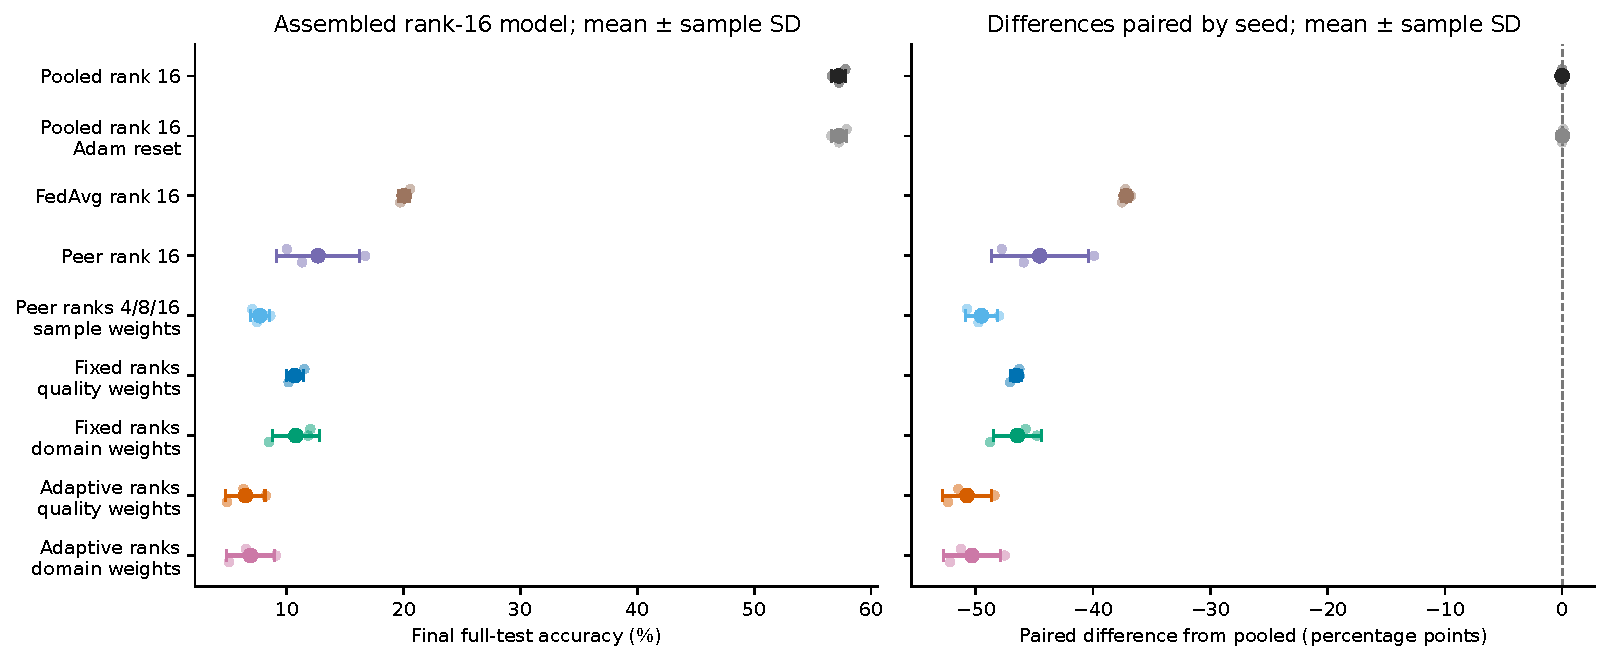
\includegraphics[width=\linewidth]{figures/integrated_final_comparison.pdf}
\caption{Corrected final rank-16 full-test comparison. All methods use the same test set; error bars show sample standard deviation across seeds 42--44. Ordinary pooled LoRA is the primary reference.}
\label{fig:integrated-final}\end{figure}
\begin{figure}[t]\centering
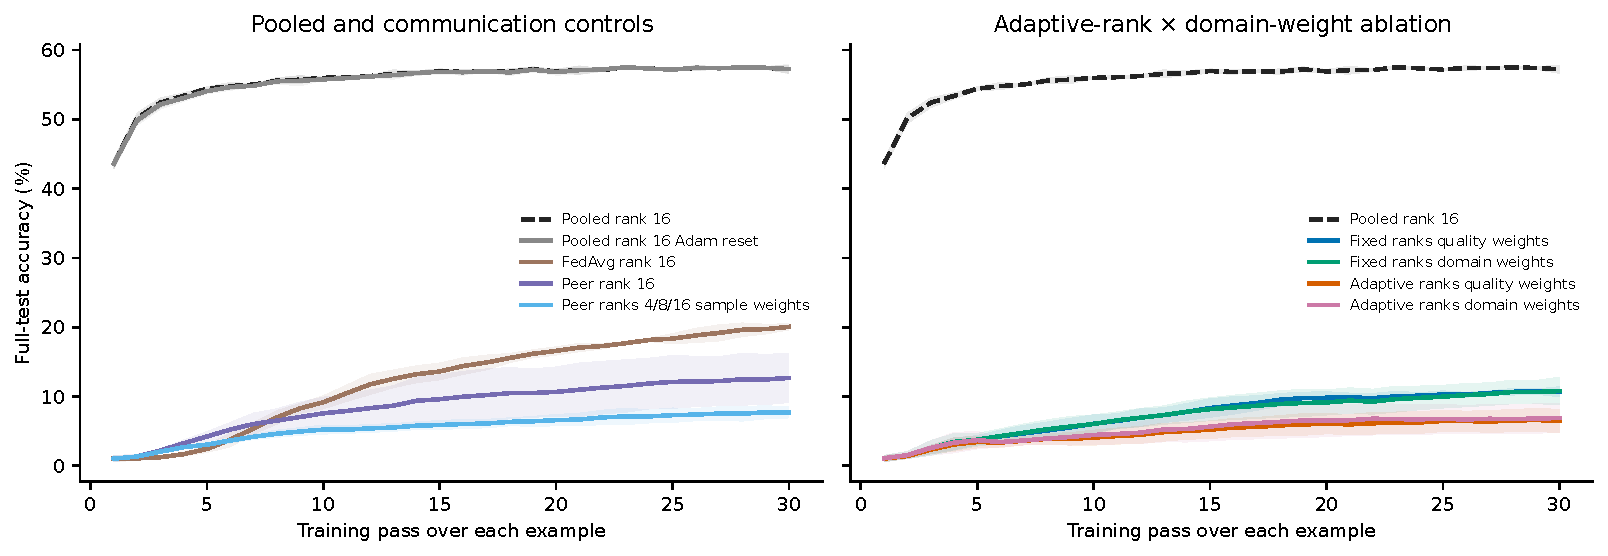
\includegraphics[width=\linewidth]{figures/integrated_accuracy_curves.pdf}
\caption{Full-test accuracy over the fixed 30-round budget. Each curve evaluates the actual deployment model at that round. Intermediate peer assembly supports evaluation only and does not feed a global model back into decentralized training.}
\label{fig:integrated-curves}\end{figure}
\begin{figure}[t]\centering
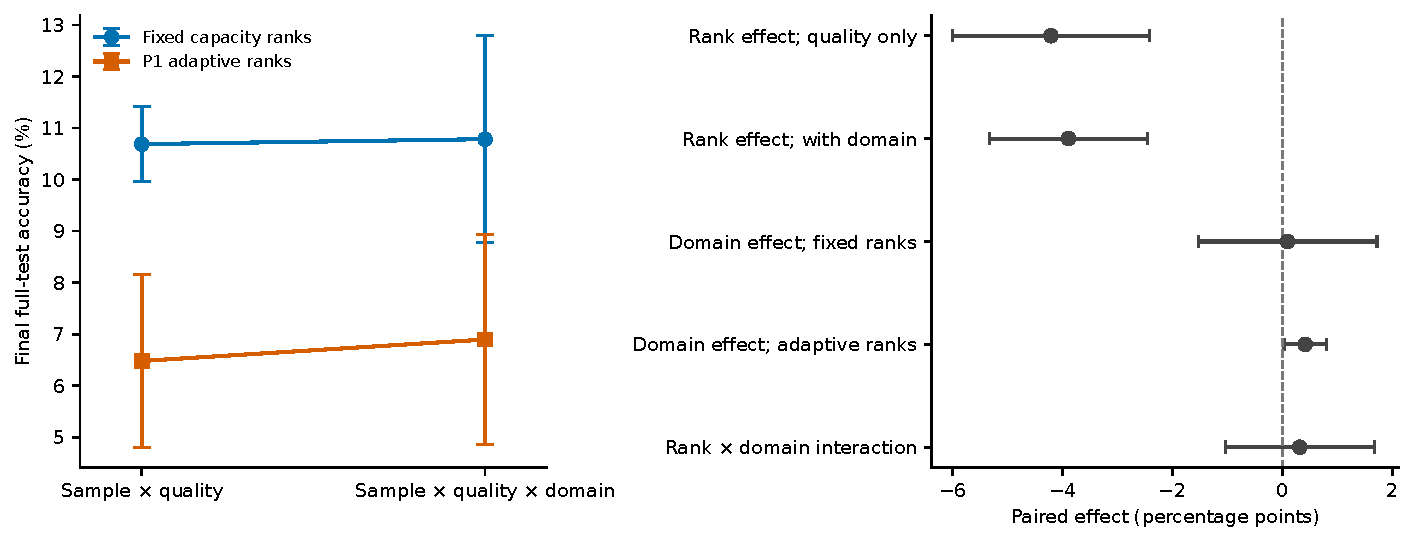
\includegraphics[width=0.9\linewidth]{figures/integrated_factorial.pdf}
\caption{Paired component effects within the corrected experiment. Rank adaptation is compared at the same weighting condition; domain factors are compared at the same rank policy. These comparisons complement the primary comparison against pooled training.}
\label{fig:integrated-factorial}\end{figure}
\begin{figure}[t]\centering
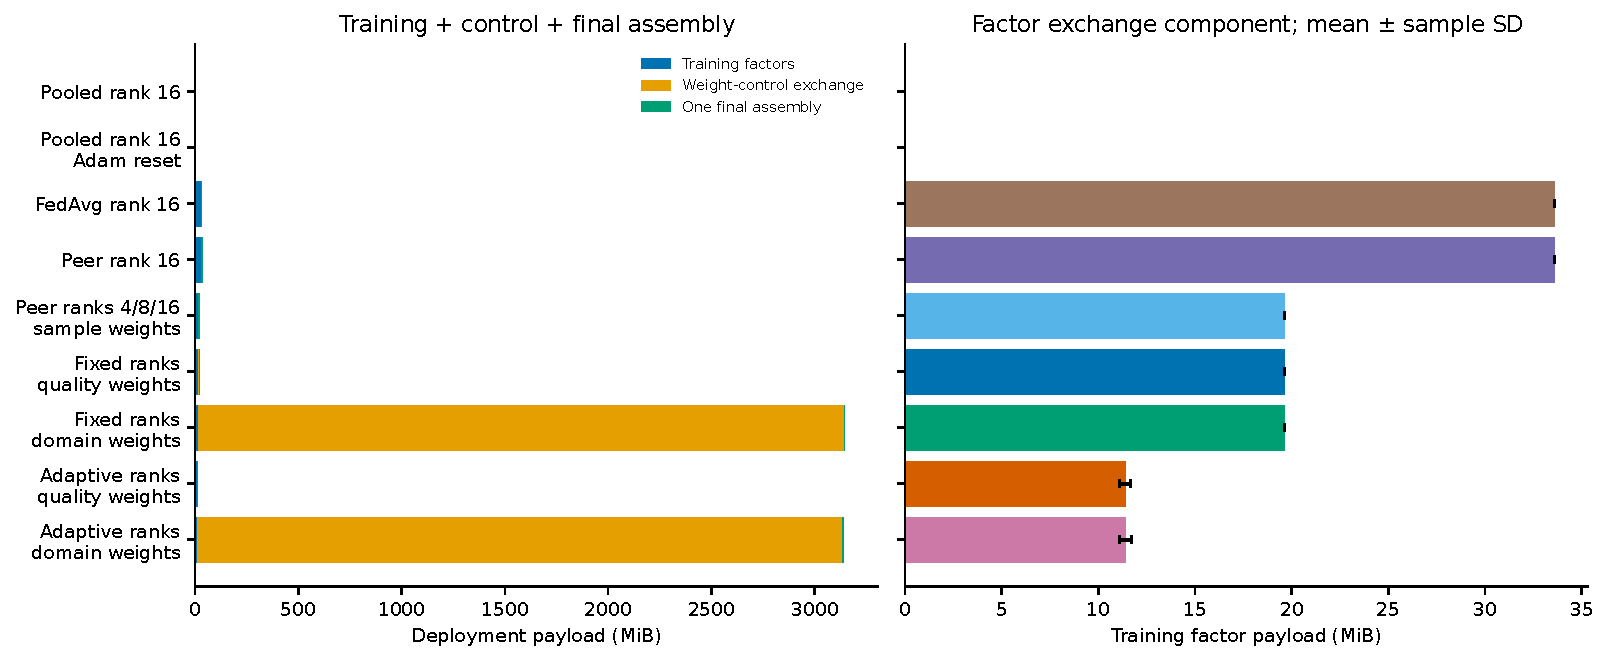
\includegraphics[width=\linewidth]{figures/integrated_communication.pdf}
\caption{Simulated deployment payload: factor exchange during training, all weighting-control traffic, and one final peer assembly. Dense control information is included. These counts are not measured bandwidth or network latency.}
\label{fig:integrated-communication}\end{figure}
\begin{figure}[t]\centering
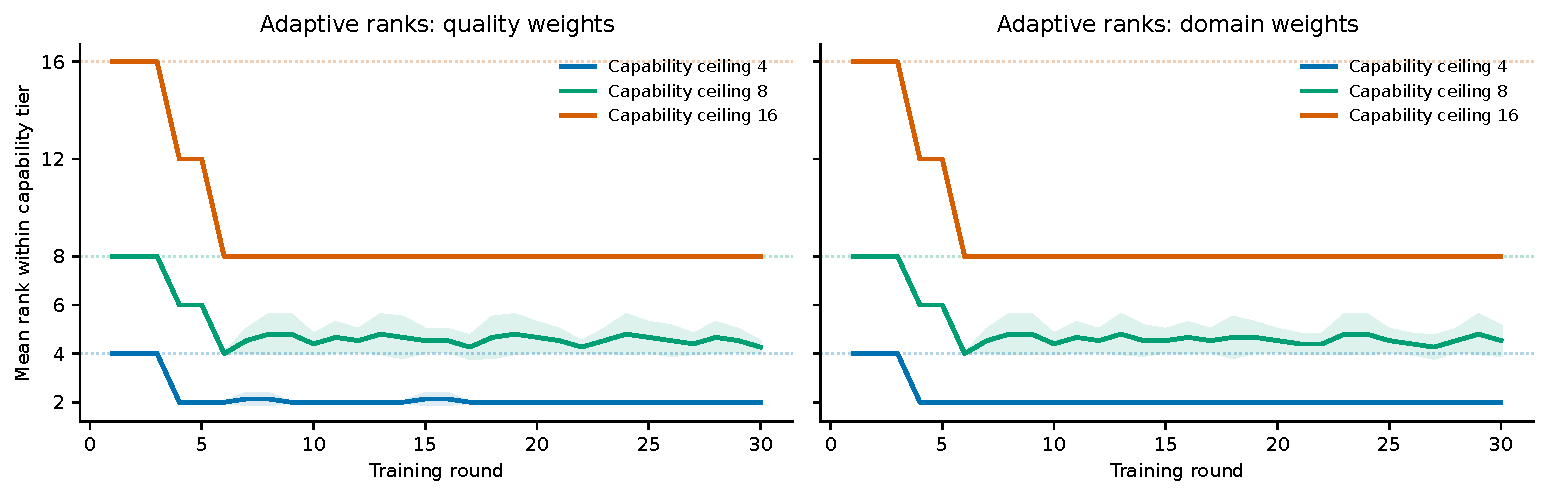
\includegraphics[width=\linewidth]{figures/integrated_rank_trajectories.pdf}
\caption{Adaptive ranks under the published capability ceilings. Rank choices and gradient probes are recorded for each client; rank reductions alone do not account for probe, SVD, or metadata costs.}
\label{fig:integrated-ranks}\end{figure}

\subsection{Label allocation explains much of the uniform-rank shortfall}
The unmodified pooled-reset and FedAvg controls reproduce the earlier scientific trajectories at all three seeds. Table~\ref{tab:optimization-controls} and Figure~\ref{fig:exploration-optimization} report the completed paired interventions. Exact rank-16 SVD after each pooled epoch changes mean final accuracy from $57.25\%$ to $57.17\%$; adding class centering also gives $57.17\%$. The maximum immediate centered-logit discrepancy on the training probes is about $4.01\times10^{-5}$. These controls do not support factor refactorization alone as the explanation for the roughly 37-point pooled--FedAvg gap.

\begin{table}[t]
\centering
\caption{Exploratory optimization controls after 30 rounds, using all 50,000 training and 10,000 test examples. Values are full-test accuracy in percent, mean $\pm$ sample SD across seeds 42--44. IID changes ownership while preserving every client's sample count.}
\label{tab:optimization-controls}
\small
\begin{tabular}{lc}
\toprule
Control & Full-test accuracy\\
\midrule
Pooled-reset & $57.25\pm0.66$\\
Pooled-reset + exact SVD & $57.17\pm0.56$\\
Pooled-reset + centering + exact SVD & $57.17\pm0.49$\\
FedAvg-16, original label skew & $20.06\pm0.44$\\
FedAvg-16 + centering & $18.51\pm1.24$\\
FedAvg-16, IID ownership & $53.25\pm0.44$\\
FedAvg-16, IID + centering & $53.30\pm0.27$\\
\bottomrule
\end{tabular}
\end{table}

Redistributing the same training examples IID raises FedAvg from $20.06\pm0.44\%$ to $53.25\pm0.44\%$, a paired increase of $33.20\pm0.84$ percentage points. A paired gap of $4.00\pm1.10$ points to pooled-reset remains. Thus severe label allocation is a major contributor under this protocol, but removing it does not demonstrate pooled parity. It also changes the original decentralized learning problem rather than providing a remedy for participants whose domains cannot be redistributed.

Class centering does not repair non-IID FedAvg: its accuracy falls to $18.51\pm1.24\%$, while IID centering gives $53.30\pm0.27\%$. The mean pre-aggregation common-logit energy fraction is 96.45\% in original FedAvg versus 2.07\% under IID ownership; this helps explain why an uncentered Frobenius denominator can obscure the geometry of the predictive update. However, the centering intervention itself does not recover accuracy. Common-mode energy is therefore a diagnostic, not a demonstrated standalone cause or successful correction.

\begin{figure}[t]\centering

\includegraphics[width=\linewidth]{figures/exploration_optimization.pdf}
\caption{Paired exploratory controls for exact factor refactorization, class centering, and training-label allocation. All endpoints use the original official test set; the IID intervention preserves dataset size and every client's sample count. These results diagnose the completed negative experiment and are not fresh confirmatory tests.}
\label{fig:exploration-optimization}\end{figure}

\subsection{Heterogeneous projection can destroy a learned model without training}
The 18 no-training runs support the information-loss mechanism in Equations~\eqref{eq:retention-recurrence} and~\eqref{eq:central-attrition}. Uniform-rank mixing preserves the pooled model's $57.23\pm0.59\%$ accuracy over 30 cycles. In contrast, initially projecting the same oracle adapter to ranks $(4,8,16)$ and assembling it gives $48.03\pm0.83\%$; repeated ring mixing and receiver projection reduce this to $13.53\pm2.32\%$ without a single optimizer step. The additional loss after initial distribution is $34.50\pm2.75$ points. The lower-rank $(2,4,8)$ stress schedule falls from $21.11\pm1.08\%$ to $5.85\pm1.63\%$.

\begin{table}[t]
\centering
\caption{Oracle-initialized information-retention test with zero training. Accuracy is measured after initial per-peer rank projection and assembly, then after 30 further mixing/projection cycles. Values are percent, mean $\pm$ sample SD over three pooled checkpoints.}
\label{tab:retention}
\small
\begin{tabular}{llcc}
\toprule
Mixing & Fixed peer ranks & Initial assembly & After 30 cycles\\
\midrule
Ring & 16 & $57.23\pm0.59$ & $57.23\pm0.59$\\
Ring & $4/8/16$ & $48.03\pm0.83$ & $13.53\pm2.32$\\
Ring & $2/4/8$ & $21.11\pm1.08$ & $5.85\pm1.63$\\
Central & 16 & $57.23\pm0.59$ & $57.23\pm0.59$\\
Central & $4/8/16$ & $48.03\pm0.83$ & $11.27\pm0.92$\\
Central & $2/4/8$ & $21.11\pm1.08$ & $4.46\pm0.24$\\
\bottomrule
\end{tabular}
\end{table}

Centralized heterogeneous averaging exhibits the same attrition (Table~\ref{tab:retention}); replacing the ring with exact averaging therefore does not by itself preserve the accumulated model when every receiver repeatedly truncates it to its own capacity. After 30 ring cycles, the $(4,8,16)$ and $(2,4,8)$ schedules retain 42.78\% and 25.78\% of the oracle adapter's energy, respectively. The comparison starts from an unavailable pooled oracle and measures robustness of an already learned state, not a federated training result. It establishes one concrete failure mechanism, without attributing the entire original accuracy gap to that mechanism.

\begin{figure}[t]\centering
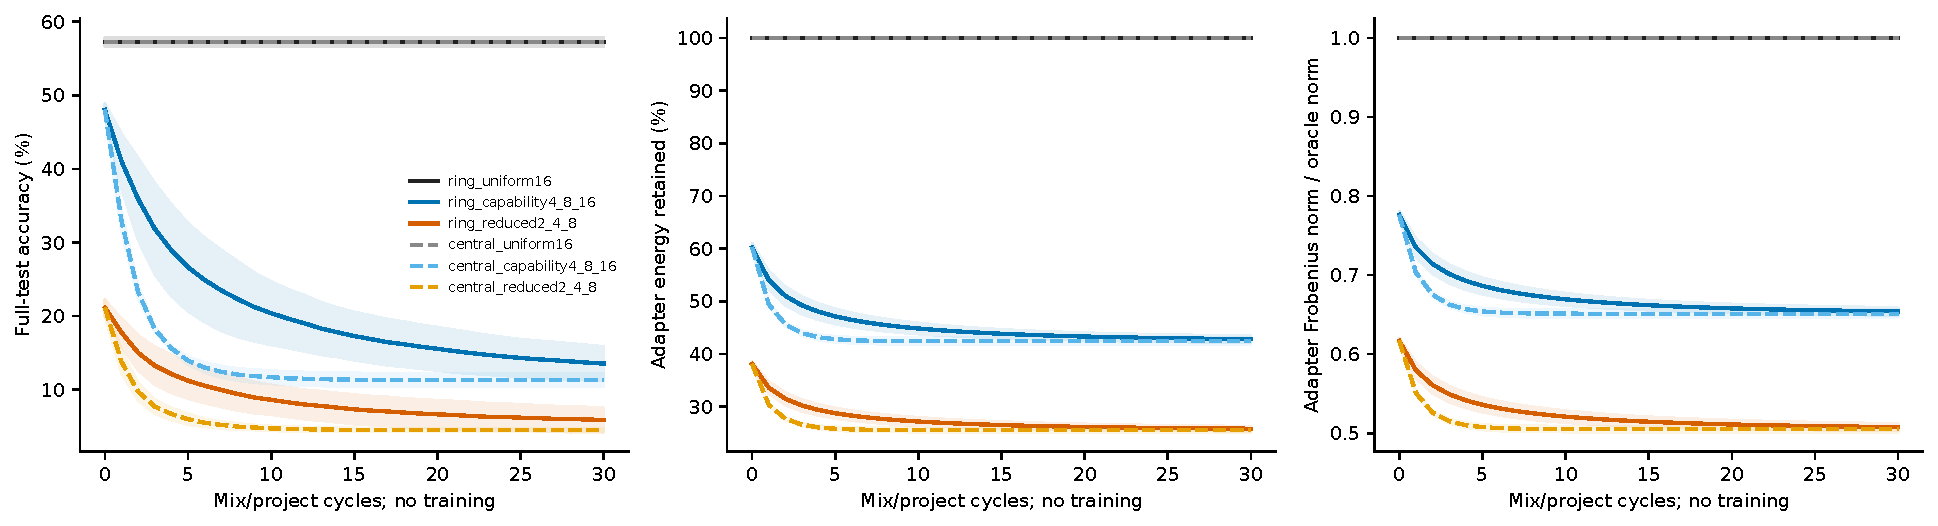
\includegraphics[width=\linewidth]{figures/exploration_rank_retention.pdf}
\caption{No-training stress test from the same completed pooled adapter at each seed. Cycle zero includes initial capacity projection and assembly. Subsequent cycles change only communication and rank projection. The uniform-rank control retains the learned classifier; repeated heterogeneous projection attenuates modes that some peers cannot store. Error bands are sample SD over three seeds.}
\label{fig:exploration-retention}\end{figure}

\subsection{Synchronized peer gradients match the pooled reference}
Exact neighbor-tree gradient synchronization reaches the same $57.23\pm0.59\%$ final accuracy as conventional pooled LoRA: the paired endpoints are 57.80\%, 56.63\%, and 57.25\% for seeds 42--44. All test predictions agree between the paired paths at every one of the 90 epoch evaluations (Figure~\ref{fig:exploration-gradient}). The factors are not bitwise identical: the largest final factor discrepancy is $5.36\times10^{-7}$. All 192 same-state fp64 gradient checks pass, with maximum absolute error $3.33\times10^{-16}$. Independent reconstruction of the forward pass reproduces all six saved checkpoint counts and prediction hashes.

This is successful numerical reproduction of the specified pooled learning path under separate data ownership and graph-restricted gradient messages. It costs 328,440 messages and 12.87 GB per run, requires rank 16 at every peer, and uses globally coordinated minibatches with common optimizer state. It therefore shows that decentralized data ownership itself need not produce the original accuracy loss, while leaving the heterogeneous-rank resource objective unresolved. It is not a claim of statistical equivalence across other tasks or of privacy.

The one-step ordering diagnostic further distinguishes gradient aggregation from aggregation after local Adam. Across 24 training minibatches, weighted local gradients agree with the pooled gradient to $6.94\times10^{-17}$, but their independently optimized effective updates have mean cosine $\chi=0.242$ with the pooled Adam update and mean relative difference $\rho=1.104$. Mean same-minibatch cross entropy falls by 0.01534 after the pooled-gradient Adam step and by 0.00144 after averaging the independent local-Adam updates. No SVD, multi-step drift, or test examples enter this diagnostic. It confirms that optimizer ordering is already consequential at one step; it does not quantify its share of the full 30-round accuracy gap.

\begin{figure}[t]\centering
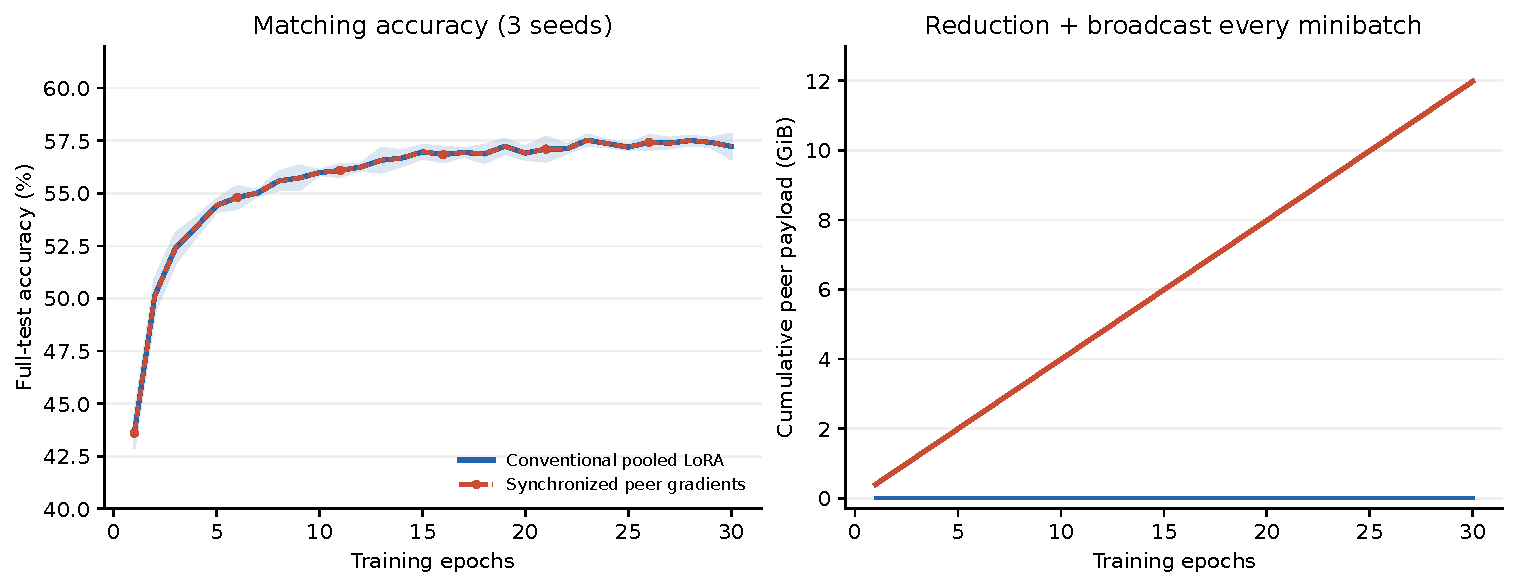
\includegraphics[width=\linewidth]{figures/exploration_gradient_equivalence.pdf}
\caption{Uniform-rank synchronized peer factor gradients reproduce the pooled training path. Full-test predictions agree at every recorded epoch for all three seeds, with small floating-point factor differences. The control uses common Adam state and a tree collective at every globally scheduled minibatch; its payload and capacity assumptions differ from adaptive one-hop gossip.}
\label{fig:exploration-gradient}\end{figure}

\subsection{Retaining a common base does not rescue the screened residual recipes}
All eight retained-base residual candidates fail the seed-42 validation screen (Figure~\ref{fig:exploration-residual}). Their final accuracies range from 1.42\% to 2.88\%, compared with 57.64\% for conventional LoRA on the same 45,000 fitting examples and 5,000 validation examples. The original fixed-domain and adaptive-domain controls reach 4.52\% and 4.62\%, respectively, on this split. These validation values have a different training budget and evaluation set from the primary full-data experiment and should not be compared as paired improvements to its endpoints.

The residual adaptive/domain recipe reaches 1.74\%, 2.64\%, and 1.48\% at gains 1, 5, and 15. At gain 5, fixed/domain reaches 2.60\%, adaptive/sample 2.88\%, and adaptive/quality 2.46\%. Uniform/sample and fixed/sample at gain 1 reach 1.68\% and 1.42\%. Thus none of the disclosed residual choices approaches the pooled reference. The gain-15 model remains finite but exhibits severe loss growth: local training cross entropy rises from 3.520 to 47.848, with a maximum of 53.490 and independently reconstructed validation cross entropy of 41.463. This is not a NaN failure or a proof of asymptotic divergence.

The zero-residual retention invariant holds algebraically, but preserving past state does not ensure that newly optimized residuals provide useful global learning. These results reject the eight tested recipes at one seed and budget rather than retained-state methods in general. Independent direct fp32 reconstruction reproduces all 11 saved checkpoint counts, including the unsuccessful and high-gain cases. The dense residual reduction and head broadcast require 164.07 MiB per 30-epoch run before quality/domain control; adding domain control raises the total to 3287.52 MiB. Smaller trainable residuals therefore neither establish the original complete-model capacity restriction nor demonstrate an efficient repair.

\begin{figure}[p]\centering
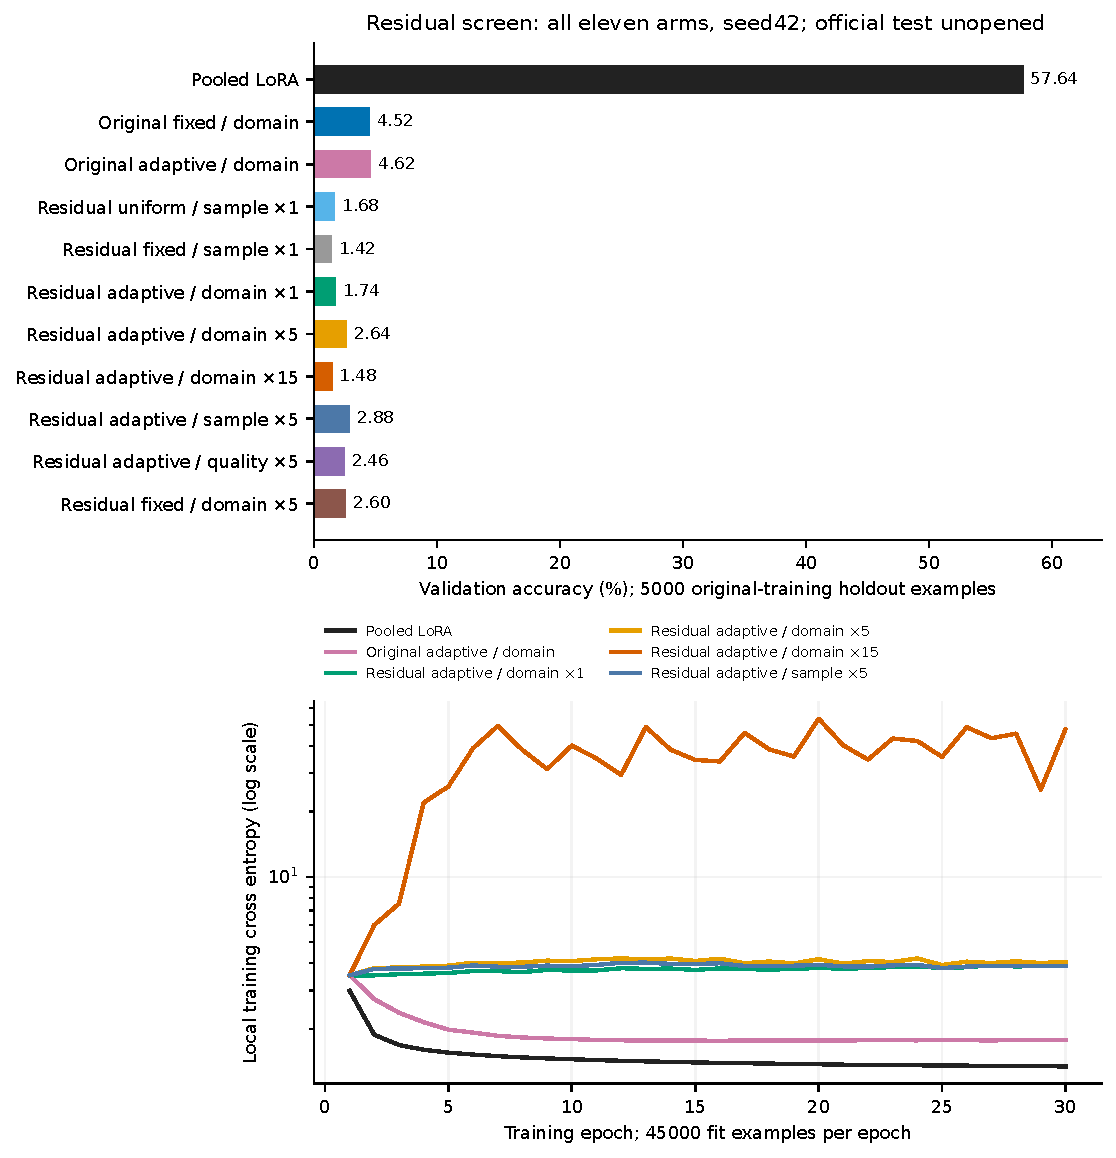
\includegraphics[width=0.87\linewidth]{figures/exploration_residual.pdf}
\caption{Completed retained-base residual screen: all eleven arms, seed 42, 30 epochs, and the common 5,000-example original-training holdout. No official-test data are opened. The upper panel retains every endpoint; the lower panel shows representative training losses, including finite instability at gain 15. Single-seed results have no between-seed error bars.}
\label{fig:exploration-residual}\end{figure}

\subsection{Partial gradients approach the reference under a different capacity model}
The shared-model variant gives a substantially stronger validation result (Table~\ref{tab:masked-results} and Figure~\ref{fig:exploration-masked}). Conventional LoRA and the uniform shared-gradient driver control both reach $57.18\pm0.71\%$ across seeds 42--44. Their independently reconstructed final prediction vectors are identical at every seed. Recorded intermediate correct counts match in 89 of 90 epoch evaluations: at seed 42, epoch 1, the uniform driver has 2058 correct predictions versus 2059 for pooled training. This validation-only analytic-gradient implementation is distinct from the earlier full-data synchronized-gradient control, whose predictions match at all 90 evaluations. Equal final predictions do not imply bitwise-identical optimization trajectories.

\begin{table}[t]
\centering
\caption{Final validation accuracy on the common 45,000/5,000 training split. Values are percent, mean $\pm$ sample SD across three paired seeds. Differences use conventional pooled LoRA on this same split as reference. Partial gradients constrain computed coordinates, not complete-model rank.}
\label{tab:masked-results}
\small
\begin{tabular}{lcc}
\toprule
Method & Validation accuracy & Paired difference (pp)\\
\midrule
Conventional pooled LoRA & $57.18\pm0.71$ & ---\\
Uniform shared-gradient control & $57.18\pm0.71$ & $0.00\pm0.00$\\
Fixed partial gradients + domain & $55.90\pm0.59$ & $-1.28\pm1.24$\\
Adaptive partial gradients + domain & $55.03\pm1.01$ & $-2.15\pm1.69$\\
\bottomrule
\end{tabular}
\end{table}

Fixed/domain partial gradients reach $55.90\pm0.59\%$, while adaptive/domain reaches $55.03\pm1.01\%$. The paired adaptive-minus-fixed difference is $-0.87\pm0.86$ percentage points. The adaptive recipe is below its fixed-budget comparator at all three seeds; it does not establish that adaptation preserves accuracy. Neither the remaining pooled gap nor its variation establishes equivalence or noninferiority without a specified margin and appropriate design.

The remaining screening contrasts have only seed 42: fixed/sample reaches 54.96\%, adaptive/sample 54.68\%, adaptive/quality 54.52\%, fixed/domain 55.26\%, and adaptive/domain 54.80\%, against 57.64\% for pooled and uniform controls. All are retained, rather than selecting only the best endpoint. The domain addition changes adaptive quality-only accuracy by 0.28 points in this single-seed screen; this does not establish a general benefit of domain allocation.

Independent evaluation reproduces all 15 partial-gradient and pooled checkpoint counts. Each run processes 1,350,000 training-example exposures and 10,560 common optimizer steps. Full rank-16 forward computation, complete factors and Adam moments, and padded rank-16 gradient transport remain required. Reduced rank--sample products measure selected gradient-coordinate work only and exclude probes, forward computation, optimizer work and aggregation. This variant shows that a changed optimization protocol can narrow the observed accuracy gap, but does not satisfy the original heterogeneous complete-model memory claim or establish privacy.

\begin{figure}[t]\centering
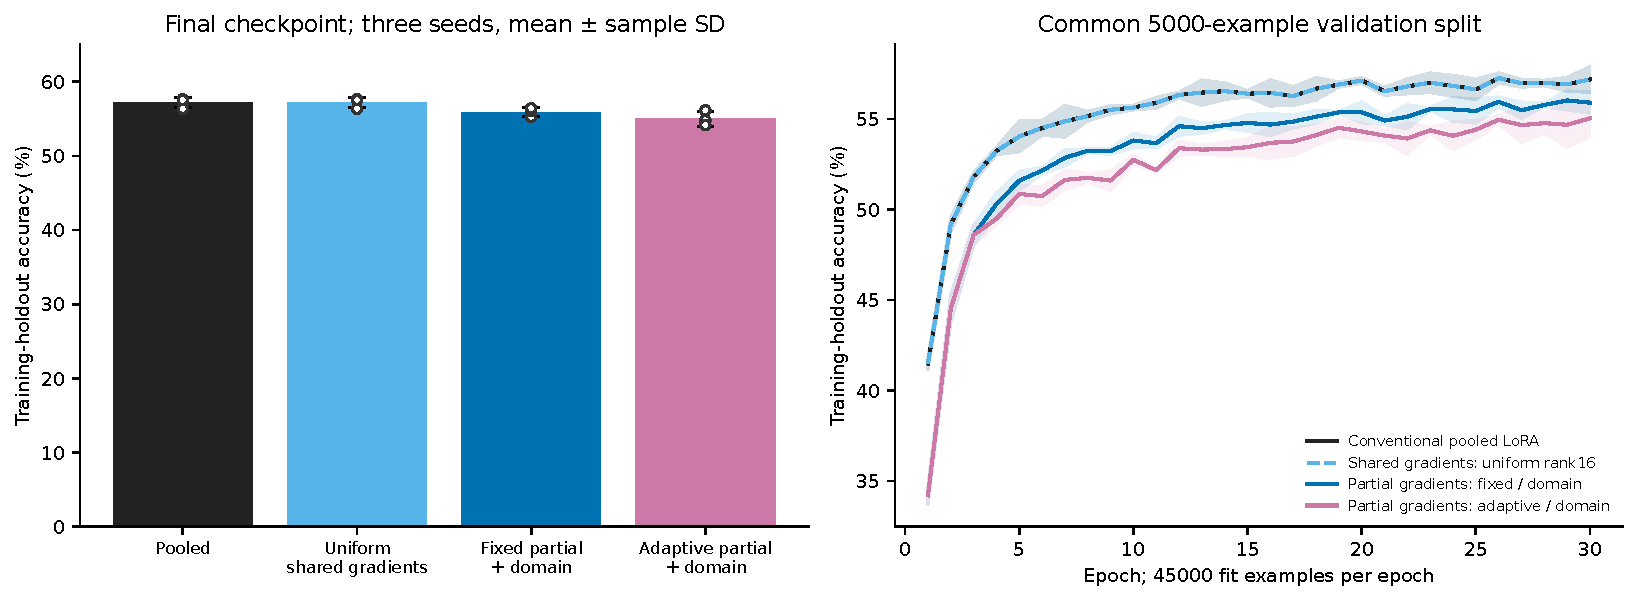
\includegraphics[width=\linewidth]{figures/exploration_masked.pdf}
\caption{Shared-model partial-gradient exploration on the fixed original-training holdout. Error bars and bands are sample SD across seeds 42--44; dots show individual endpoints. The uniform driver and conventional pooled curves nearly overlap and share final prediction vectors. Fixed and adaptive partial-gradient variants retain full rank-16 model, forward and optimizer state despite their smaller gradient-coordinate budgets.}
\label{fig:exploration-masked}\end{figure}

\subsection{What the component evidence establishes}
Table~\ref{tab:historical-protocols} retains the earlier 50-round protocol results. With uniform rank 16, the oracle hierarchy reaches $68.98\pm0.95\%$ personalized accuracy, while its diagnostic consensus accuracy is $10.25\pm0.62\%$. This contrast illustrates why a domain-specific personalized score cannot establish parity of one globally deployed model. The oracle result remains useful evidence that known domain structure changes the behavior of local models.

\begin{table}[t]
\centering
\caption{Supporting historical Project 3 results after 50 rounds, in percent (mean $\pm$ sample standard deviation, seeds 42--44). The objective is client-uniform; historical consensus is an evaluator-assembled uniform average. These values are not the corrected pooled comparison.}
\label{tab:historical-protocols}
\small
\begin{tabular}{llcc}
\toprule
Rank context & Method & Personalized & Diagnostic consensus\\
\midrule
Uniform 16 & Local & $57.93\pm0.55$ & $14.23\pm1.27$\\
& FedAvg & $23.20\pm0.29$ & $23.20\pm0.29$\\
& MH & $42.30\pm1.39$ & $15.14\pm5.10$\\
& Oracle hierarchy & $68.98\pm0.95$ & $10.25\pm0.62$\\
\midrule
Heterogeneous $4/12/32$ & Local & $53.60\pm0.62$ & $14.50\pm0.80$\\
& FedAvg & $5.74\pm0.71$ & $5.73\pm0.59$\\
& MH & $28.45\pm2.42$ & $6.83\pm0.45$\\
& Oracle hierarchy & $44.07\pm0.70$ & $11.47\pm1.13$\\
\bottomrule
\end{tabular}
\end{table}

Under the historical heterogeneous schedule, factor zero-padding gives personalized accuracy of $4.71\pm0.22\%$ for FedAvg, $20.63\pm4.40\%$ for MH, and $31.24\pm1.27\%$ for the oracle hierarchy, compared with $44.07\pm0.70\%$ for effective-update oracle mixing. Error feedback gives $26.63\pm1.68\%$ for MH and $41.28\pm0.71\%$ for the oracle. These are finite-run ablations of representation and compression, not universal performance orderings.

The separate online-discovery experiment selects five groups with adjusted Rand index $1.00$ at stage 10 for each seed. At stage 20 its scores are $1.00$, $0.918$, and $1.00$, with the middle seed selecting six groups. This demonstrates recovery under coordinator-visible observations; it neither establishes a privacy property nor substitutes for the fixed-ring pooled comparison.

The original Project 1 controller stayed at rank 2 throughout its five-round battery and reduced the reported training-FLOP estimate by 93.75\% against fixed rank 32, while losing accuracy on three of five tasks. Since rank 32 violates every tested client ceiling, that comparison does not measure a feasible hardware-matched accuracy trade-off. The revised Fashion-MNIST rerun finishes at 82.85\% for both the adaptive controller and feasible fixed ranks $(4,8,16)$, with a reported 10.0\% reduction in the training-FLOP estimate. This is one task, one seed, and five rounds; its unscaled adapter convention also differs from the corrected scaled-head benchmark.

Project 2's conservative follow-up changes Spearman association with recorded contributions from 0.152 to 0.196 and pairwise ordering accuracy from 0.520 to 0.547. These are model-free ranking results, not retrained-model accuracy results. Its earlier ridge forms have weak global fit ($R^2=0.079$ and $0.025$) and task-dependent correlations. Neither the isolated Fashion-MNIST parity nor the contribution-ranking change predicts the composed method's full-test accuracy without the corrected experiment.

\section{Discussion and Limitations}
The parity question has several distinct comparisons. Pooled versus FedAvg tests the effect of local optimization and aggregation with uniform rank. MH-16 adds neighbor communication. MH-sample imposes heterogeneous capacity. The four quality/domain arms then isolate the selected adaptive policy and the domain multipliers. A shortfall at one step cannot automatically be attributed to a different component, and matching a resource-constrained federated control does not establish matching pooled training.

The follow-up experiments replace a generic failure diagnosis with several narrower findings. Label redistribution recovers more than 33 points of uniform-rank FedAvg accuracy, while exact pooled SVD refactorization changes its pooled control by less than one tenth of a point on average. Removing common-logit offsets does not restore non-IID accuracy. The no-training test establishes repeated heterogeneous model projection as an independent mechanism for destroying retained information. The one-step Adam test shows that aggregation after local optimization can differ substantially from optimization after gradient aggregation even with no multi-step drift or SVD. These interventions identify effects in their respective settings; their magnitudes cannot be added to explain the original full-pipeline gap.

The earlier small Frobenius diagnostics remain valid but were insufficient to identify these mechanisms. FedAvg's mean per-round relative discarded energy is $1.39\times10^{-6}$, and the final adaptive-domain assembly discards a mean relative energy of $7.63\times10^{-5}$. Neither statistic measures all predictive information removed over earlier rounds, and the uncentered norm can be dominated by a softmax-invariant offset. The uniform-rank peer arm also reaches $42.10\pm1.42\%$ personalized accuracy while its full-test assembled model reaches $12.69\pm3.55\%$, illustrating local specialization rather than accuracy of one globally useful model.

Equal global sample exposures, even with all optimizer steps counted, do not make local-then-average training equivalent to pooled sequential optimization. Local objectives differ, Adam's gradient transformation depends nonlinearly on its moments, and SVD refactorization changes factor coordinates before the next optimizer reset. In general, if $\mathcal U_i$ is a local optimization map and $\mathcal U_{\rm pool}$ its pooled counterpart,
\begin{equation}
 \mathcal C_R\left(\sum_i\pi_i\mathcal U_i(\dW)\right)
 \ne \mathcal U_{\rm pool}(\dW).
\end{equation}
This explains why the desired equality is an empirical hypothesis rather than an algebraic property of weighted assembly. Even in a first-order SGD approximation, one local epoch with $\tau_i$ local steps gives a sample-weighted change proportional to $\sum_i(n_i/n)\tau_i\nabla f_i$, so variable $\tau_i$ changes the effective contribution of local trajectories. That approximation is not an exact description of Adam. The synchronized-gradient control establishes a sufficient route to reproduce pooled optimization, but jointly changes synchronization frequency, gradient aggregation order, and shared optimizer state. It does not identify a unique cause of FedAvg's shortfall.

The successful uniform-rank positive control changes the scope of the conclusion: the evidence rejects the tested adaptive state-averaging protocol, not the proposition that decentralized data ownership can coexist with pooled accuracy. It nevertheless leaves the original resource claim open because every synchronized peer stores the full rank-16 model and optimizer. The completed candidate studies sharpen this distinction. All screened retained-base recipes remain far below their pooled validation reference, despite preserving a frozen accumulated model. Partial-gradient training reaches within 2.15 points on average under adaptive/domain allocation, but its fixed/domain comparator performs better, and it reduces computed gradient coordinates without reducing full model or Adam storage. Neither method satisfies the original complete-model rank cap merely because its local computation uses a smaller $r_i$.

The benchmark deliberately exposes costs that a factor-only account omits. Domain weighting currently exchanges dense update changes and class histograms with every peer, and final exact assembly also uses dense matrices. This simple protocol makes data dependencies auditable but can dominate the savings from smaller factor payloads. A compressed sufficient-statistic protocol would be a different implementation requiring its own correctness and accuracy evaluation. Rank--sample products likewise omit gradient probes, factorization, optimizer work, and dense processing.

The execution is a single-process simulation of peer message flow on the designated remote GPU machine. It verifies graph-constrained operations and payloads; it does not establish multi-host reliability, measured communication speed, asynchronous behavior, or tolerance of dropped clients. The cached-feature, head-only CIFAR-100 task does not validate end-to-end visual fine-tuning, language models, medical data, or arbitrary AI training. Three seeds describe variation in this testbed and do not establish broad equivalence. The official-test mechanism controls are exploratory follow-ups to an observed failure; the later 45,000/5,000 split limits further selection to training data but does not erase that research history. The historical oracle and automatic-discovery results have different observation assumptions and are not silently included in the corrected pipeline.

Raw examples are absent from the simulated peer messages, and each client's optimizer reads its assigned examples. The simulator process nevertheless has access to the entire dataset, so this experiment does not verify enforced isolation between machines. Updates and training statistics are exposed; in particular, the domain-control allgather reveals all supplied records to all peers. No differential privacy, secure aggregation, membership-inference evaluation, reconstruction evaluation, or medical threat model is implemented in this study. Consequently, accuracy parity, if observed, would still not justify a claim that hospitals can collaborate without privacy loss.

\section{Conclusion}
The original adaptive-rank, domain-weighted state-averaging protocol is unsuccessful at preserving pooled accuracy: its corrected 30-round result is $6.90\pm2.03\%$ against $57.23\pm0.59\%$ for conventional rank-16 LoRA. The completed follow-up experiments make this conclusion more specific. Severe label skew accounts for much of the uniform-rank FedAvg shortfall, optimizer aggregation order changes even a single local step, and repeated heterogeneous projection can erase a learned classifier without training. Exact synchronized peer gradients reproduce the pooled reference at every evaluated epoch, establishing that separate data ownership need not itself cause accuracy loss. That positive control requires full rank 16, common Adam state, and 12.87 GB of modeled communication per run. On a separate training-only validation split, all eight retained-base residual recipes fail, while adaptive partial gradients reach $55.03\pm1.01\%$ against $57.18\pm0.71\%$ for pooled LoRA. This narrower gap is obtained by retaining full rank-16 model and optimizer state, and fixed partial gradients perform better than adaptive ones. The original joint claim of pooled accuracy under complete-model heterogeneous rank caps therefore remains unsupported; the evidence supports further protocol research rather than declaring decentralized LoRA impossible. No tested protocol establishes a privacy guarantee for the proposed hospital use case.

\appendix
\section{Reproducibility and Supporting Figures}
The repository contains executable protocols, canonical policy provenance, feature and split hashes, per-round JSON records, phase timings, final adapters, and scripts that generate the reported tables and plots. The corrected driver is \path{project-3-hierarchical-gossip/experiments/integrated_benchmark.py}. Its evaluation does not tune on test data. Remote tests cover the numerical operators and paired execution invariants; artifacts distinguish full experiments from smoke tests and excluded pilots. Local credentials are not part of the artifact bundle.

The follow-up evidence is stored under \path{docs/artifacts/methodology-exploration/}, with prospective plans separating official-test diagnostics from validation-only candidate exploration. Optimization controls retain all 21 endpoints and independently reconstructed correct counts; retention runs preserve spectra, coefficient recurrence predictions, and all 18 no-training trajectories. The gradient control preserves six paired final models, 192 same-state fp64 checks, and independent predictions and communication counts. The Adam-order diagnostic retains all 24 training-only probes. Residual and partial-gradient verifiers independently reconstruct 25 unique saved validation models (11 residual-screen and 15 partial-gradient/pooled evaluations share one pooled checkpoint), with every correct count matching. They open only the original training tensor, validate its hash and exhaustive class-stratified holdout, and check exposures, initialization, rank ceilings, weight formulas and recorded transport ledgers. Per-step gradient edge traces are not retained, so their actual runtime paths cannot be independently reconstructed from the saved counters. A 47-file snapshot is verified against the six validation launch manifests and canonical P1/P2 dependency hashes. All unsuccessful candidates, the finite high-gain instability, raw per-round records and checkpoints remain archived. Figure files in the paper directory are copied from remotely generated artifacts rather than manually plotted from selected outcomes. Historical figures below retain their original protocols and should be read with the associated qualifications.

\begin{figure}[p]
\centering
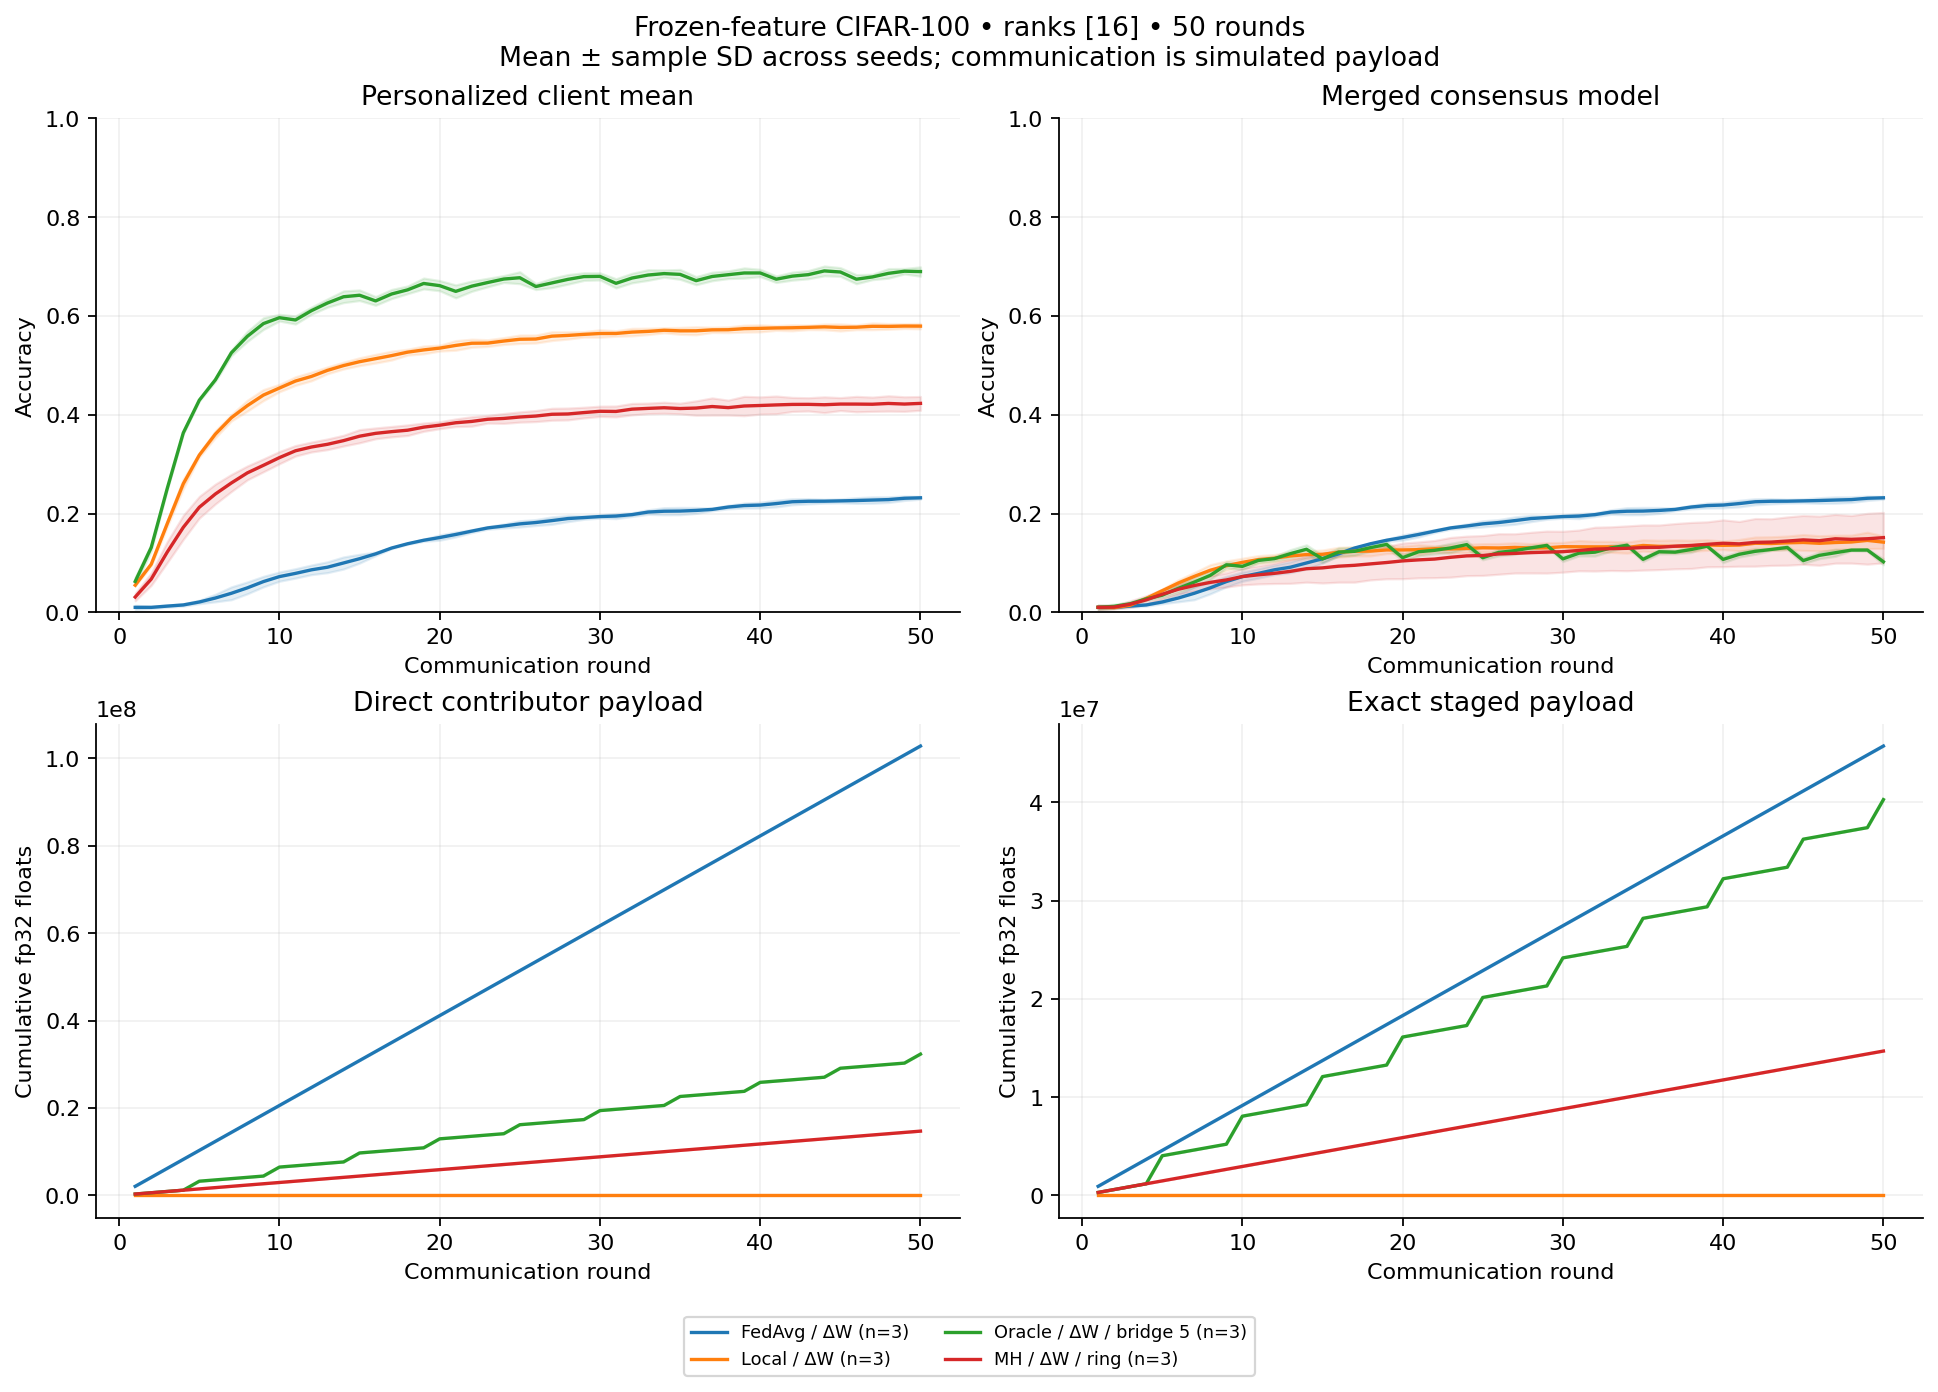
\includegraphics[width=\linewidth]{figures/p3_uniform_curves.png}
\caption{Supporting historical uniform-rank protocol curves, 50 rounds. Personalized and evaluator-assembled consensus accuracy are different endpoints.}
\label{fig:historical-uniform}
\end{figure}
\begin{figure}[p]
\centering
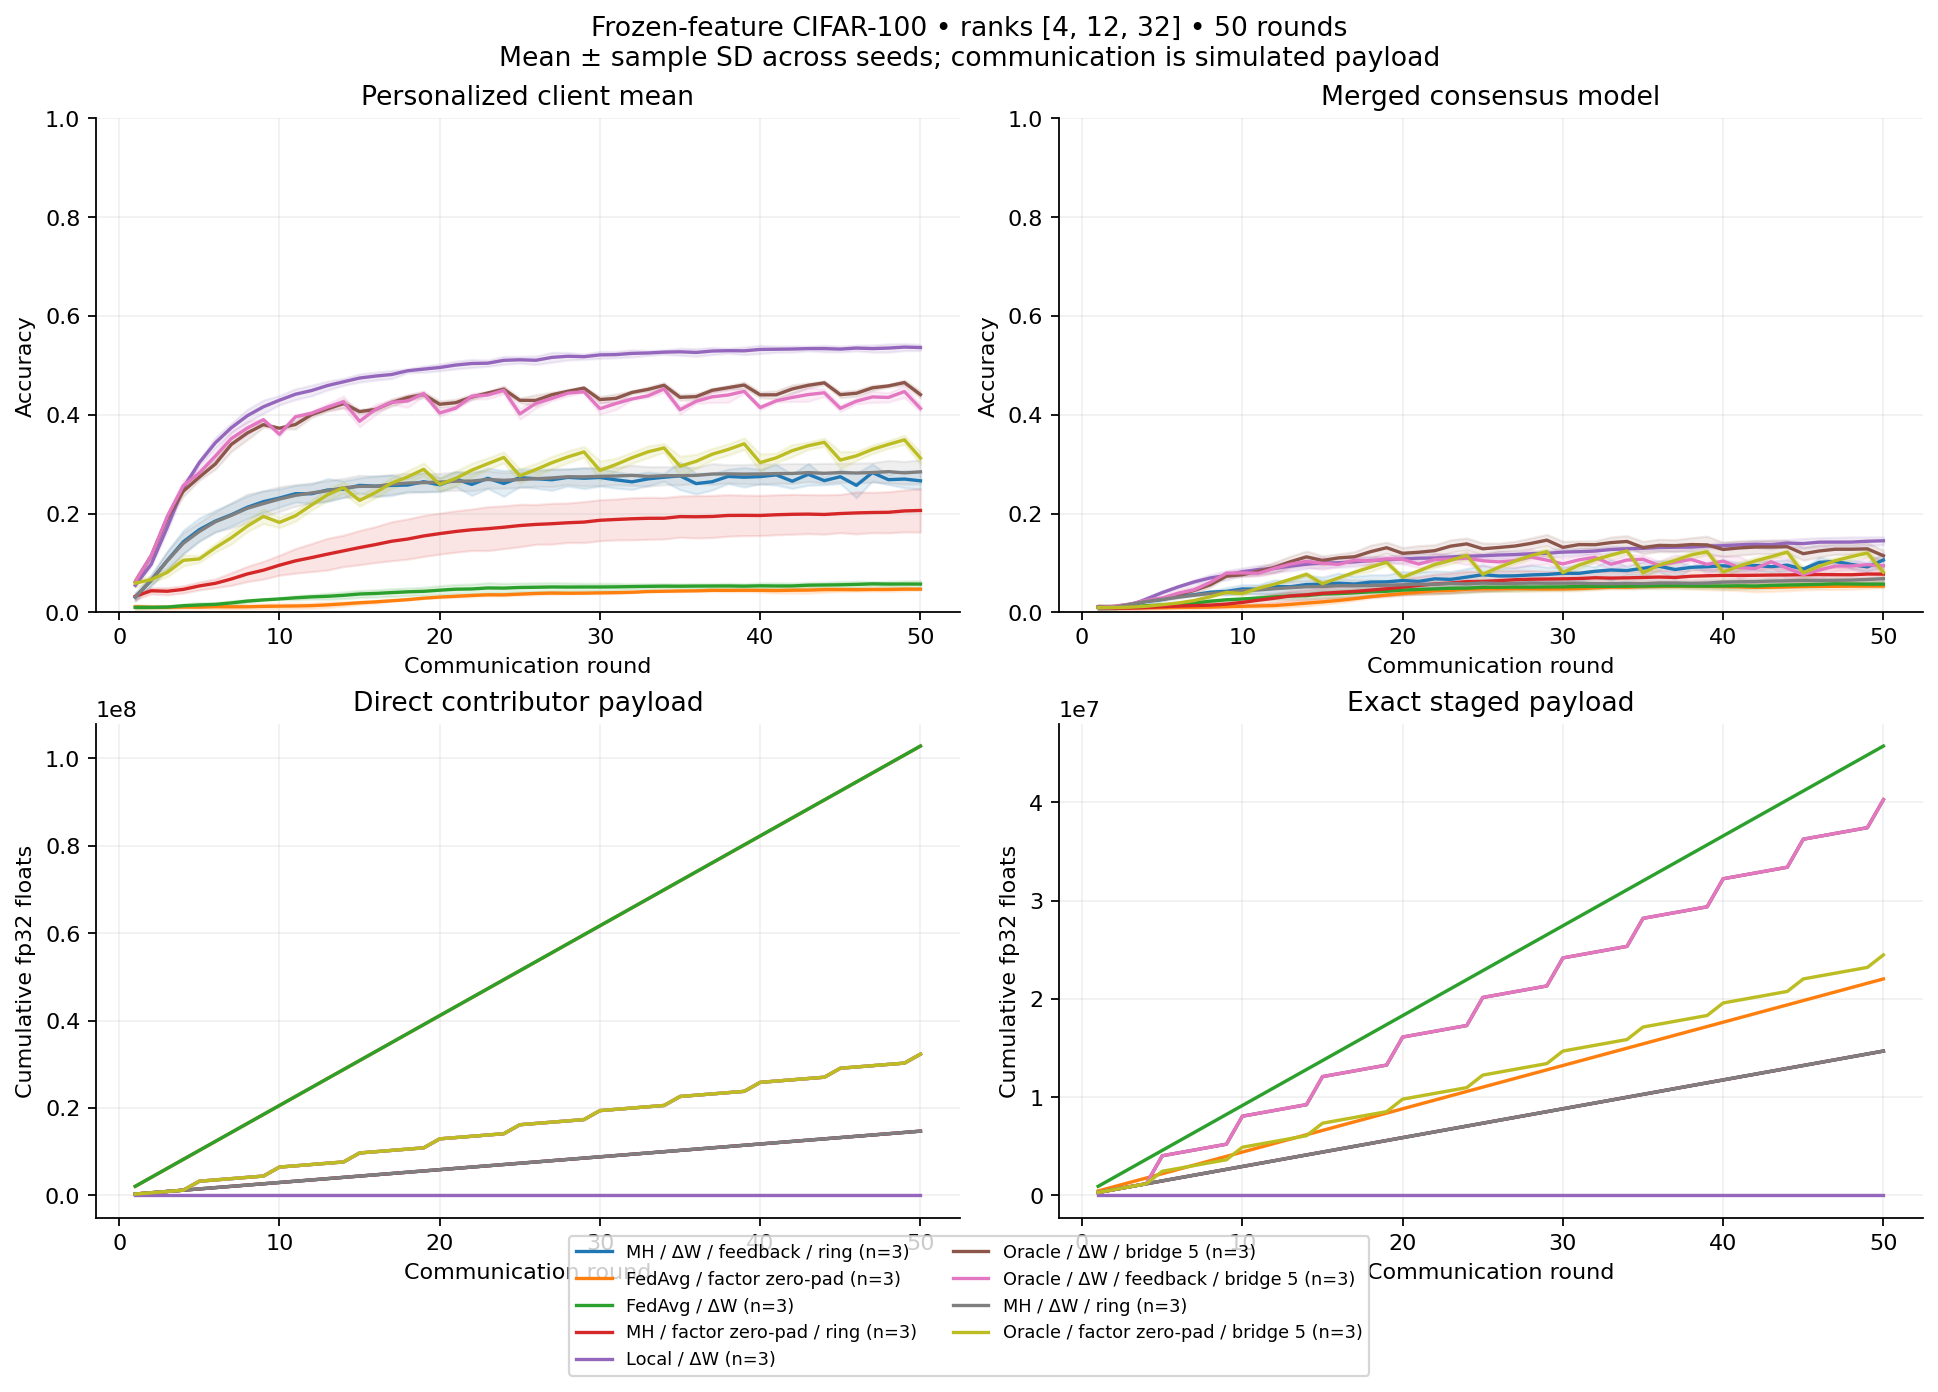
\includegraphics[width=\linewidth]{figures/p3_heterogeneous_curves.png}
\caption{Supporting historical heterogeneous $(4,12,32)$ protocol curves. The rank budget and objective differ from the corrected $(4,8,16)$ pooled comparison.}
\label{fig:historical-heterogeneous}
\end{figure}
\begin{figure}[p]
\centering
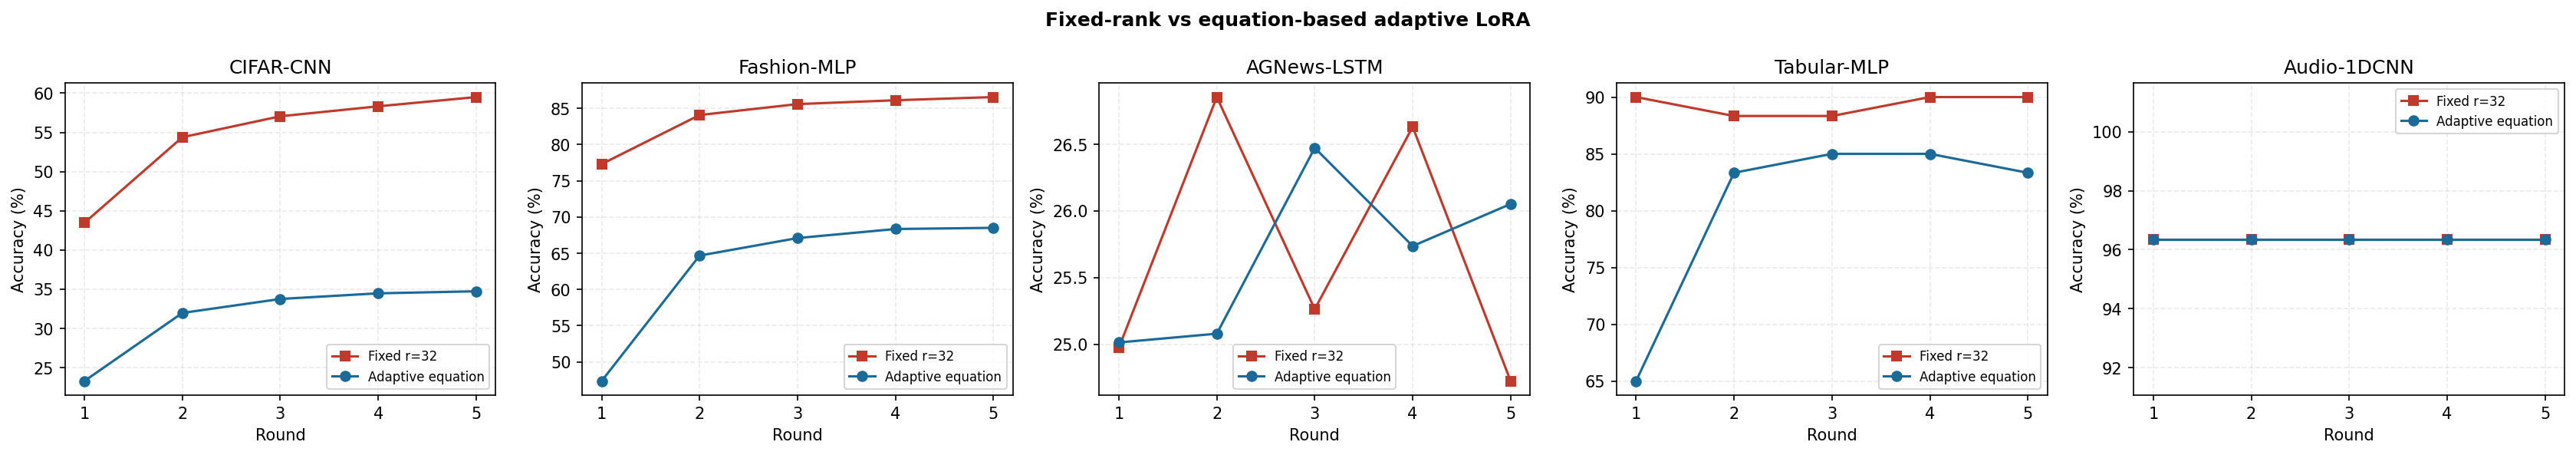
\includegraphics[width=\linewidth]{figures/p1_adaptive_accuracy_curves.png}
\caption{Historical five-task Project 1 battery. Fixed rank 32 exceeds the tested capability ceilings and is not a feasible hardware-matched reference. The revised Fashion-MNIST comparison is reported separately.}
\label{fig:historical-p1}
\end{figure}
\begin{figure}[p]
\centering
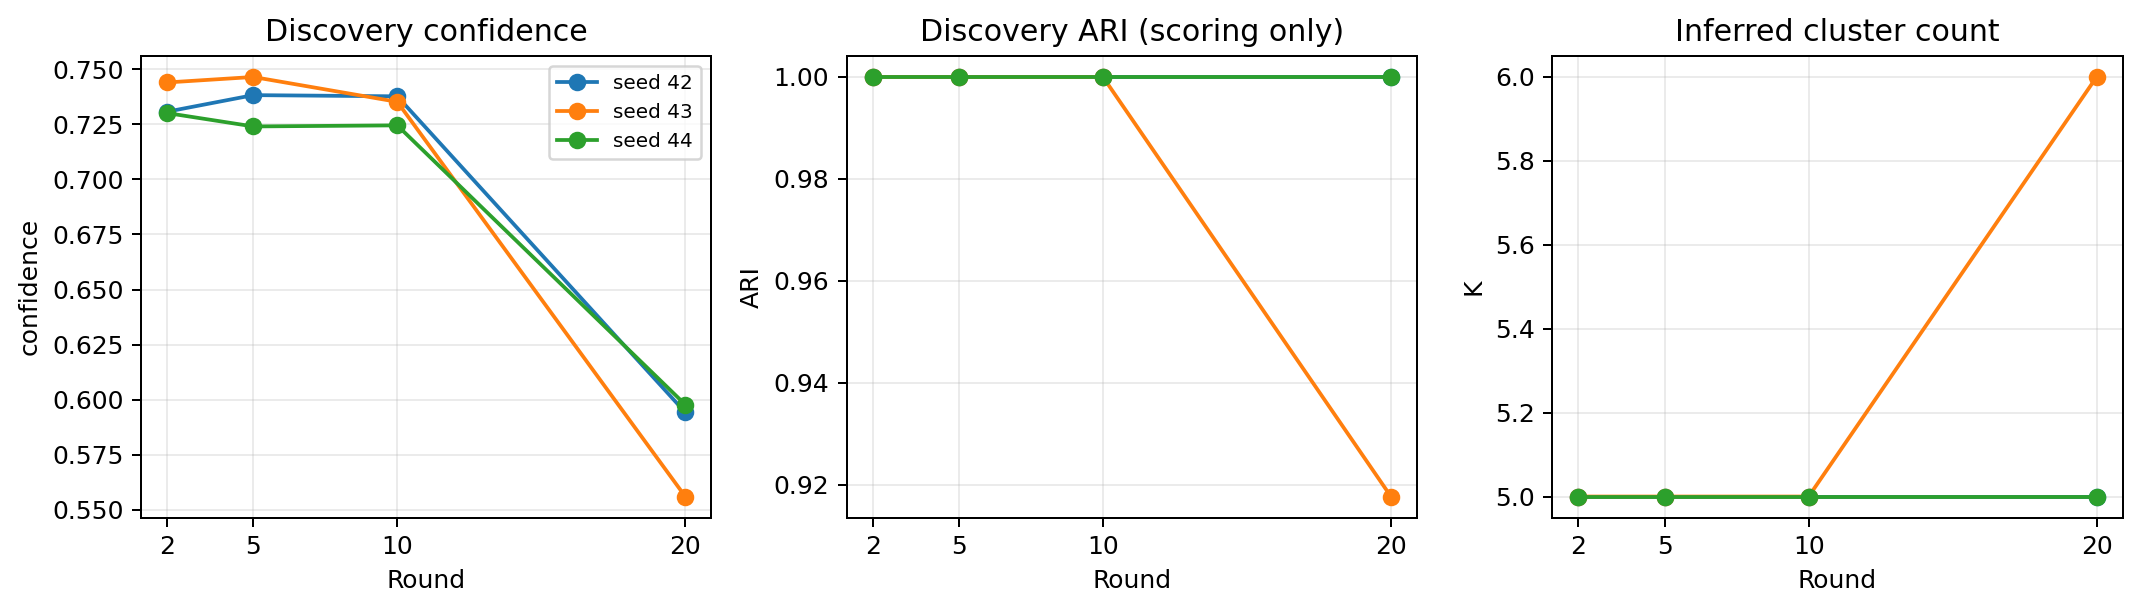
\includegraphics[width=\linewidth]{figures/p3_adaptive_discovery.png}
\caption{Supporting online-discovery results under coordinator-visible adapter observations. This experiment evaluates group recovery and is separate from the corrected fixed-ring pipeline.}
\label{fig:historical-discovery}
\end{figure}
\clearpage
\bibliographystyle{plainnat}
\bibliography{references}
\end{document}
